%%%%%%%%%%%%%%%%%%%%%%%%%%%%%%%%%%%%%%%%%%%%%%%%%%%%%%%%%%%%%%%
%% OXFORD THESIS TEMPLATE

% Use this template to produce a standard thesis that meets the Oxford University requirements for DPhil submission
%
% Originally by Keith A. Gillow (gillow@maths.ox.ac.uk), 1997
% Modified by Sam Evans (sam@samuelevansresearch.org), 2007
% Modified by John McManigle (john@oxfordechoes.com), 2015
% Modified by Ulrik Lyngs (ulrik.lyngs@cs.ox.ac.uk), 2018, for use with R Markdown
%
% Ulrik Lyngs, 25 Nov 2018: Following John McManigle, broad permissions are granted to use, modify, and distribute this software
% as specified in the MIT License included in this distribution's LICENSE file.
%
% John tried to comment this file extensively, so read through it to see how to use the various options.  Remember
% that in LaTeX, any line starting with a % is NOT executed.  Several places below, you have a choice of which line to use
% out of multiple options (eg draft vs final, for PDF vs for binding, etc.)  When you pick one, add a % to the beginning of
% the lines you don't want.


%%%%% CHOOSE PAGE LAYOUT
% The most common choices should be below.  You can also do other things, like replacing "a4paper" with "letterpaper", etc.

% This one will format for two-sided binding (ie left and right pages have mirror margins; blank pages inserted where needed):
%\documentclass[a4paper,twoside]{templates/ociamthesis}
% This one will format for one-sided binding (ie left margin > right margin; no extra blank pages):
%\documentclass[a4paper]{ociamthesis}
% This one will format for PDF output (ie equal margins, no extra blank pages):
%\documentclass[a4paper,nobind]{templates/ociamthesis}
%UL 2 Dec 2018: pass this in from YAML
\documentclass[a4paper, twoside]{templates/ociamthesis}

% add hyperref package with options from YAML %
\usepackage[colorlinks=false,pdfpagelabels,hidelinks]{hyperref}

% add float package to allow manual control of figure positioning %
% this was taken from the stackoverflow answer at: https://stackoverflow.com/a/33801326/14802285 %
\usepackage{float}
\let\origfigure\figure
\let\endorigfigure\endfigure
\renewenvironment{figure}[1][2] {
    \expandafter\origfigure\expandafter[H]
} {
    \endorigfigure
}

%UL set section header spacing
\usepackage{titlesec}
\titleformat{\chapter}
  {\normalfont\Large\bfseries}{\thechapter}{1em}{}
\titlespacing*{\chapter}{0pt}{3.5ex plus 1ex minus .2ex}{2.3ex plus .2ex}
% 
\titlespacing\subsubsection{0pt}{24pt plus 4pt minus 2pt}{0pt plus 2pt minus 2pt}

% UL 30 Nov 2018 pandoc puts lists in 'tightlist' command when no space between bullet points in Rmd file
\providecommand{\tightlist}{%
  \setlength{\itemsep}{0pt}\setlength{\parskip}{0pt}}
 
% UL 1 Dec 2018, fix to include code in shaded environments

%UL set whitespace around verbatim environments
\usepackage{etoolbox}
\makeatletter
\preto{\@verbatim}{\topsep=0pt \partopsep=0pt }
\makeatother

%UL 26 Mar 2019, enable strikethrough
\usepackage[normalem]{ulem}

%UL use soul package for correction highlighting
\usepackage{color, soul}
\usepackage{xcolor}
\definecolor{correctioncolor}{HTML}{CCCCFF}
\sethlcolor{correctioncolor}
\newcommand{\ctext}[3][RGB]{%
  \begingroup
  \definecolor{hlcolor}{#1}{#2}\sethlcolor{hlcolor}%
  \hl{#3}%
  \endgroup
}
\soulregister\ref7
\soulregister\cite7
\soulregister\autocite7
\soulregister\textcite7
\soulregister\pageref7

% user-included things with header_includes or in_header will appear here
% kableExtra packages will appear here if you use library(kableExtra)
\usepackage{booktabs}
\usepackage{longtable}
\usepackage{array}
\usepackage{multirow}
\usepackage{wrapfig}
\usepackage{float}
\usepackage{colortbl}
\usepackage{pdflscape}
\usepackage{tabu}
\usepackage{threeparttable}
\usepackage{threeparttablex}
\usepackage[normalem]{ulem}
\usepackage{makecell}
\usepackage{xcolor}


%%%%%%% PAGE HEADERS AND FOOTERS %%%%%%%%%
\usepackage{fancyhdr}
\setlength{\headheight}{15pt}
\fancyhf{} % clear the header and footers
\pagestyle{fancy}
\renewcommand{\chaptermark}[1]{\markboth{\thechapter. #1}{\thechapter. #1}}
\renewcommand{\sectionmark}[1]{\markright{\thesection. #1}} 
\renewcommand{\headrulewidth}{0pt}

\fancyhead[LO]{\emph{\leftmark}} 
\fancyhead[RE]{\emph{\rightmark}} 

% UL page number position 
\fancyfoot[C]{\emph{\thepage}} %regular pages
\fancypagestyle{plain}{\fancyhf{}\fancyfoot[C]{\emph{\thepage}}} %chapter pages

% JEM fix header on cleared pages for openright
\def\cleardoublepage{\clearpage\if@twoside \ifodd\c@page\else
   \hbox{}
   \fancyfoot[C]{}
   \newpage
   \if@twocolumn\hbox{}\newpage
   \fi
   \fancyhead[LO]{\emph{\leftmark}} 
   \fancyhead[RE]{\emph{\rightmark}} 
   \fi\fi}


%%%%% SELECT YOUR DRAFT OPTIONS
% This adds a "DRAFT" footer to every normal page.  (The first page of each chapter is not a "normal" page.)

% This highlights (in blue) corrections marked with (for words) \mccorrect{blah} or (for whole
% paragraphs) \begin{mccorrection} . . . \end{mccorrection}.  This can be useful for sending a PDF of
% your corrected thesis to your examiners for review.  Turn it off, and the blue disappears.
\correctionstrue

% IP feb 2021: option to include line numbers in PDF

%%%%% BIBLIOGRAPHY SETUP
% Note that your bibliography will require some tweaking depending on your department, preferred format, etc.
% If you've not used LaTeX before, I recommend reading a little about biblatex/biber and getting started with it.
% If you're already a LaTeX pro and are used to natbib or something, modify as necessary.
% Either way, you'll have to choose and configure an appropriate bibliography format...



\usepackage{natbib}
\setcitestyle{authoryear}
\bibliographystyle{templates/myplainnat.bst}
\addto\captionsenglish{%
  \renewcommand{\bibname}{References}
}

% This makes the bibliography left-aligned (not 'justified') and slightly smaller font.
\renewcommand*{\bibfont}{\raggedright\small}


% Uncomment this if you want equation numbers per section (2.3.12), instead of per chapter (2.18):
%\numberwithin{equation}{subsection}


%%%%% THESIS / TITLE PAGE INFORMATION
% Everybody needs to complete the following:
\title{Using a Coupled Radiative Transfer Model and Artifical Neural Networks to Retrieve Forest Biochemical and Biophysical Maps from Remote Sensing Data}
\author{Author:\\
Zavud Baghirov (1399020)\\
~\\
Supervisors:\\
Prof.~Dr.~Thomas Udelhoven\\
Dr.~Martin Schlerf}
\college{}

% Master's candidates who require the alternate title page (with candidate number and word count)
% must also un-comment and complete the following three lines:

% Uncomment the following line if your degree also includes exams (eg most masters):
%\renewcommand{\submittedtext}{Submitted in partial completion of the}
% Your full degree name.  (But remember that DPhils aren't "in" anything.  They're just DPhils.)
\degree{Environmental Science}
% Term and year of submission, or date if your board requires (eg most masters)
\degreedate{Winter Semester 2021}


%%%%% YOUR OWN PERSONAL MACROS
% This is a good place to dump your own LaTeX macros as they come up.

% To make text superscripts shortcuts
	\renewcommand{\th}{\textsuperscript{th}} % ex: I won 4\th place
	\newcommand{\nd}{\textsuperscript{nd}}
	\renewcommand{\st}{\textsuperscript{st}}
	\newcommand{\rd}{\textsuperscript{rd}}

%%%%% THE ACTUAL DOCUMENT STARTS HERE
\begin{document}

%%%%% CHOOSE YOUR LINE SPACING HERE
% This is the official option.  Use it for your submission copy and library copy:
\setlength{\textbaselineskip}{22pt plus2pt}
% This is closer spacing (about 1.5-spaced) that you might prefer for your personal copies:
%\setlength{\textbaselineskip}{18pt plus2pt minus1pt}

% You can set the spacing here for the roman-numbered pages (acknowledgements, table of contents, etc.)
\setlength{\frontmatterbaselineskip}{17pt plus1pt minus1pt}

% UL: You can set the line and paragraph spacing here for the separate abstract page to be handed in to Examination schools
\setlength{\abstractseparatelineskip}{13pt plus1pt minus1pt}
\setlength{\abstractseparateparskip}{0pt plus 1pt}

% UL: You can set the general paragraph spacing here - I've set it to 2pt (was 0) so
% it's less claustrophobic
\setlength{\parskip}{2pt plus 1pt}

%
% Customise title page
%
\def\crest{{
\includegraphics[scale=0.6]{templates/uni-logo.png}}}
\renewcommand{\university}{Department of Environmental Remote Sensing and Geoinformatics\\
~\\
University of Trier}
\renewcommand{\submittedtext}{Submitted in partial fulfillment of the requirements for the degree of Master of Science in}
\renewcommand{\thesistitlesize}{\fontsize{18pt}{28pt}\selectfont}


% Leave this line alone; it gets things started for the real document.
\setlength{\baselineskip}{\textbaselineskip}


%%%%% CHOOSE YOUR SECTION NUMBERING DEPTH HERE
% You have two choices.  First, how far down are sections numbered?  (Below that, they're named but
% don't get numbers.)  Second, what level of section appears in the table of contents?  These don't have
% to match: you can have numbered sections that don't show up in the ToC, or unnumbered sections that
% do.  Throughout, 0 = chapter; 1 = section; 2 = subsection; 3 = subsubsection, 4 = paragraph...

% The level that gets a number:
\setcounter{secnumdepth}{2}
% The level that shows up in the ToC:
\setcounter{tocdepth}{2}


%%%%% ABSTRACT SEPARATE
% This is used to create the separate, one-page abstract that you are required to hand into the Exam
% Schools.  You can comment it out to generate a PDF for printing or whatnot.

% JEM: Pages are roman numbered from here, though page numbers are invisible until ToC.  This is in
% keeping with most typesetting conventions.
\begin{romanpages}

% Title page is created here
\maketitle

%%%%% DEDICATION -- If you'd like one, un-comment the following.

%%%%% ACKNOWLEDGEMENTS -- Nothing to do here except comment out if you don't want it.


%%%%% ABSTRACT -- Nothing to do here except comment out if you don't want it.
\begin{abstract}
	This will be the abstract at the end {[}TO BE UPDATED{]}
\end{abstract}

%%%%% MINI TABLES
% This lays the groundwork for per-chapter, mini tables of contents.  Comment the following line
% (and remove \minitoc from the chapter files) if you don't want this.  Un-comment either of the
% next two lines if you want a per-chapter list of figures or tables.

% This aligns the bottom of the text of each page.  It generally makes things look better.
\flushbottom

% This is where the whole-document ToC appears:
\tableofcontents

\listoffigures
	\mtcaddchapter
  	% \mtcaddchapter is needed when adding a non-chapter (but chapter-like) entity to avoid confusing minitoc

% Uncomment to generate a list of tables:
\listoftables
  \mtcaddchapter
%%%%% LIST OF ABBREVIATIONS
% This example includes a list of abbreviations.  Look at text/abbreviations.tex to see how that file is
% formatted.  The template can handle any kind of list though, so this might be a good place for a
% glossary, etc.
% First parameter can be changed eg to "Glossary" or something.
% Second parameter is the max length of bold terms.
\begin{mclistof}{List of Abbreviations}{3.2cm}

\item[3D] Three-dimensional
\item[INFORM] Invertable Forest Reflectance Model
\item[RTM] Radiative Transfer Model
\item[SAIL] Scattering by Arbitrary Inclined Leaves
\item[PROSAIL] The combination of PROSPECT and SAIL models
\item[FLIM] Forest Light Interaction Model
\item[LAI] Leaf Area Index
\item[MLRA] Machine Learning Regression Algorithms
\item[ML] Machine Learning
\item[DT] Decision Trees
\item[ANN] Artificial Neural Networks
\item[KBMLRM] Kernel-Based Machine Learning Regression Methods
\item[RF] Random Forest
\item[RFR] Random Forest Regression
\item[LUT] Look-Up-Table
\item[NN] Neural Networks
\item[SVR] Support Vector Regression
\item[SVM] Support Vector Machines
\item[GPR] Gaussian Process Regression
\item[GP] Gaussian Process
\item[VI] Vegetation Index
\item[DR] Dimensionality Reduction
\item[WT] Wavelet Tranform
\item[PCA] Principal Component Analysis
\item[AL] Active Learning

\end{mclistof} 


% The Roman pages, like the Roman Empire, must come to its inevitable close.
\end{romanpages}

%%%%% CHAPTERS
% Add or remove any chapters you'd like here, by file name (excluding '.tex'):
\flushbottom

% all your chapters and appendices will appear here
\hypertarget{introduction}{%
\chapter{Introduction}\label{introduction}}

Forests cover approximately 30\% of the earth's surface and play a critical role in the water and carbon cycles \citep{laurent2011inversion}. As forest environments are being threatened more and more, there is an increased concern for forest conservation \citep{grammatikopoulou2021value}. The effects of climate change on many different ecosystems have been studied and shown. Forest ecosystems are particularly more sensitive to climate change compared to other ecosystems \citep{esquivel2019compositional, lindner2010climate}. According to \citet{lindner2010climate}, the primary reason forest ecosystems are particularly susceptible to extraordinary climate changes is because, in comparison to other organisms, trees typically live longer and have fewer adaptive abilities to cope with rapid environmental changes.

Another threat to the forest that has been increasingly reported during the last century is insect disturbances. Insect disturbances have increased the concern about forest species diversity, biogeochemical cycle and the economic value of forest ecosystems \citep{senf2017remote}. The main forest insects that are responsible for many outbreaks can be divided into bark beetles and defoliators. Many bark beetle species can reproduce their offspring within both dead and living tree organisms' phloem. These bark beetles can easily destroy the structure of translocation processes (e.g.~water and nutrient translocations) by introducing various pathogens (e.g.~fungal) into healthy trees \citep{senf2017remote}.

A study by \citet{kautz2017biotic} has reported that there is only a limited amount of consistent data for studying forest disturbance caused by insects \citep{senf2017remote}. Remote sensing images provide very interesting insights into studying environmental disturbances and changes within forest areas. According to the study by \citet{lechner2020applications}, remote sensing techniques have recently been actively used for forest studies. For example, remote sensing images are offering important opportunities to map ecosystem distribution, to study forest plant productivity and to get insights about the 3D structural properties of forest plants \citep{lechner2020applications}.

One of the most important insights remote sensing provides is the fact that the image of the earth's surface can be acquired over time. This gives a unique opportunity to be able to study environmental changes in a specific area of interest over the time period the images are acquired. For example, there have been studies where remote sensing techniques were used to map the distribution of invasive species and to monitor land changes (e.g.~forest habitat fragmentation) in forests \citep{lechner2020applications}.

Another interesting opportunity that remote sensing data provides is to estimate vegetation biophysical and biochemical properties from remotely sensed images. Essentially, there are various ways to retrieve plant biophysical parameters from remote sensing data. Each method has its own advantages and disadvantages. The radiative transfer model (RTM) has been accepted to be the superior method to all the available techniques \citep{darvishzadeh2019analysis, wang2018mapping}. Various RTMs have been proposed at different scales, such as leaf and canopy scales. Different RTMs such as leaf and canopy can be used in a coupled mode in order to simulate canopy reflectance based on vegetation biophysical and biochemical properties \citep{morcillo2019quantifying}.

There are mainly three inversion methods to estimate plant traits from remote sensing data. These methods are numerical optimization, look-up-table and hybrid techniques. Numerical optimization is considered to be a classical method. However, the major drawbacks of this method are its computational inefficiency and the high risk of poor convergence \citep{zhang2021analyzing}. The LUT method refers to a technique where databases to store simulated data are created by RTMs. And then, plant biophysical variables of the simulated reflectance that represent the measured data most closely are chosen as retrievals. Although the LUT method is more efficient than the classic numerical optimization, it is still a computationally inefficient process given that inversion needs to be done for each pixel in the remote sensing product \citep{danner2021efficient}. The hybrid method can be used to overcome the challenges of these less efficient techniques. In a typical hybrid method, a regression model is combined with RTMs \citep{zhang2021analyzing}.

Invertable Forest Reflectance Model (INFORM) is a combination of three RTMs (leaf and canopy) that can be used to simulate forest canopy reflectance in terms of canopy biophysical and biochemical parameters \citep{atzberger2000development, schlerf2006inversion}. INFORM and machine learning models can be combined using a hybrid method to retrieve plant traits.

The main objectives of this study are to:

\begin{enumerate}
\def\labelenumi{\arabic{enumi}.}
\tightlist
\item
  simulate forest canopy reflectance (for the national park Hunsrück-Hochwald) using the more recent submodels of the coupled chain RTM INFORM
\item
  train Artificial Neural Networks (ANN) using the simulated canopy reflectance data in order to assess whether the relationship between plant traits and spectral data can be efficiently learned
\item
  assess whether the trained ANN can deal with collinearity occurring in hyperspectral remote sensing data
\item
  retrieve forest biophysical and biochemical maps for the study area Hunsrück-Hochwald
\end{enumerate}

\hypertarget{forest-disturbances-by-bark-beetle}{%
\chapter{Forest Disturbances by Bark Beetle}\label{forest-disturbances-by-bark-beetle}}

Insect disturbance is just one of the numerous natural disturbances that forests face. Insect outbreaks can have a significant impact on the functioning of an ecosystem \citep{raffa2009literal}. However, there have been concerns regarding these forest disturbances as severity and frequency of these disturbances have increased \citep{millar2015temperate}.

One of the major insect contributors to European forest disturbances is called the European spruce bark beetle (\emph{Ips typographus}). These bark beetles have been increasingly destroying European forests. These pest organisms specifically affects Norway spruce forests, as \emph{Ips typographus}s are major pests of Norway spruce trees \citep{ohrn2014seasonal}. Temperature has a significant effect on the successful swarm of \emph{Ips typographus}. The temperature of 16.5\(^\circ\) is considered to be the minimum temperature (lower threshold) for the bark beetle to swarm and attack the trees. The length of warm days is another factor increasing the chance of successful attack by the bark beetle. The European spruce trees have defense mechanisms to fight against the mass beetle outbreak. However, when there are at least three warm days in a row with a temperature well-above the swarming threshold of \emph{Ips typographus}, then the likelihood of these pest organisms successfully overcoming the defense mechanisms of the trees and infesting them is higher \citep{wermelinger2004ecology}.

Once a tree is infested, there are typically three stages that the tree will go through. These stages are called the green attack, red attack and gray attack stages \citep{sprintsin2011combining}. The green attack stage is the first stage and it refers to a stage where usually the leaves of the infested trees are still green. At this stage, it is difficult to distinguish the infested trees at the canopy level \citep{wulder2006estimating}. During the green attack stage, the infested tree may still be alive, but once this stage has started, the death of the infested tree is inevitable. Moreover, during this stage, the freshly hatched generation of the bark beetle uses the inner bark of the tree to grow and develop \citep{niemann2005assessment}. The next stage is called the red attack stage. During this phase, the leaves of the infested trees slowly turn yellow and eventually become reddish \citep{fernandez2020monitoring}. The red attack stage occurs within the next year (one year) after the bark beetles perform a mass attack \citep{niemann2005assessment}. The final stage is the gray attack stage, which refers to a stage where the trees have already shed their leaves \citep{wulder2009challenges}. At this point, the infested trees are completely dead and abandoned by the new generation of the bark beetle \citep{niemann2005assessment}. During the final stage, typically only the gray bark of the tree is left. Hence, this stage is called the gray stage \citep{abdullah2019sensitivity}.

Bark beetles are known to have a mutual (symbiotic) relationship with many different fungi species (e.g.~\emph{Ceratocystis spp}). These fungi species can easily infect trees. Sapwood and phloem of the trees are specifically affected by these species \citep{niemann2005assessment, six2003genetic}. Once the trees are infected by the fungi carried by bark beetles, these fungi will start to disrupt the translocation of water and important nutrients in the infected tree \citep{paine1997interactions, wermelinger2004ecology}. These are potentially causing changes in both biophysical and biochemical properties at the canopy and leaf level \citep{abdullah2018european}.

There are several factors that help \emph{Ips typographus} to attack trees successfully. One of the major contributors to this process is thought to be climate change. Typically, when bark beetles exist at natural and low densities, they cannot overcome the defense mechanisms of the trees. Climate change, on the other hand, is facilitating these beetles' successful attack in numerous ways. Increased length and number of warm and very dry days, for example, significantly increase the likelihood of a mass bark beetle outbreak. Specifically, these factors trigger beetle attacks in two ways: directly (e.g.~increased insect population) and indirectly (e.g.~weakened tree defence mechanisms against bark beetle) \citep{bale2002herbivory, bentz2015modeling, marini2017climate}.

Effective forest management and early intervention is essential in order to deal with bark beetle outbreaks. Detecting the infested trees while they are still going through the green attack stage is essential, because at this point, the beetles have not yet left the tree to look for new host trees. One of the traditional ways of identifying and assessing infested trees is through manual field surveys. Typically, these surveys are performed by foresters who try to look for sawdust within the bark of the trees. However, this method is extremely difficult, time-consuming and require a lot of labor to study large forest areas. The field of remote sensing, however, offers methods to more effectively detect and map forest infestations \citep{abdullah2019sentinel, immitzer2014early}.

\citet{immitzer2014early} used World-View-2 data in order to study and detect bark beetle infestations during the green attack stage. In this study, a forest infestation map was produced using a machine learning method. Study by \citet{ortiz2013early} used RapidEye and TerraSAR-X data for early detection of bark beetle. This study demonstrated the use of statistical and machine learning methods for bark beetle detection. \citet{lausch2013forecasting} used hyperspectral airborne data HyMap to study early detection of bark beetle infestations with a limited amount of success. In the study by \citet{lausch2013forecasting}, single and multi-date Landsat data were successfully utilized to study forest disturbance by the bark beetle.

There have only been limited studies assessing the effect of the bark beetle green attack stage on plant biophysical and biochemical properties. A study by \citet{abdullah2018european} showed that there is a significant difference in leaf chlorophyll and nitrogen content between healthy and infested trees during the green attack stage. This study also concluded that spectral responses (using in-situ data) between healthy and infested trees were significantly different. Work by \citet{abdullah2019sentinel} concluded that the leaf chlorophyll and water content of healthy plants were significantly higher than infested trees at the green attack stage. They found dry matter content to be significantly higher for infested trees than healthy trees. A recent study by \citet{ali2021canopy} for the first time demonstrated the use of canopy chlorophyll content time series data retrieved from multispectral remote sensing data using the INFORM RTM for bark beetle infestation detection.

\hypertarget{rtm}{%
\chapter{Radiative Transfer Models (RTM)}\label{rtm}}

Radiative transfer models take advantage of physical laws that determine ``causal and effect'' relationships. There have been various radiative transfer models developed (leaf, canopy etc.) during the last decades \citep{verrelst2019quantifying}.

\citet{combal2003retrieval} describe that RTM inversion process involves modifying the vegetation biophysical parameters (variables) \(V = \{V_{1}, V_{2}, ..., V_{n_{var}}\}\) in such a way that the simulated canopy reflectance simulated by an RTM \(M\) is most similar to the canopy reflectance \(R\) measured by a remote sensing sensor. The \(n_{var}\) number of canopy variables and geometric parameters \(C\) are required by the RTM \(M\). It is also important to mention that the inversion is achieved with an error or uncertainty, namely \(\varepsilon\):

\begin{equation}
R\ =\ M\left(V,\ C\right)\ +\varepsilon
\label{eq:rtm}
\end{equation}

The error term \(\varepsilon\) in the Equation \eqref{eq:rtm} refers to the uncertainties in both measured and modeled canopy reflectance \citep{combal2003retrieval}.

Radiative transfer models can be used to retrieve forest canopy biophysical and biochemical variables from remote sensing satellite data. This chapter mainly focuses on a coupled-chain radiative transfer model called the Invertable Forest Reflectance Model (INFORM) and its sub-models. INFORM combines leaf and canopy radiative transfer models \citep{atzberger2000development}, namely PROSPECT, SAIL (Scattering by Arbitrary Inclined Leaves) and FLIM (Forest Light Interaction Model) models \citep{schlerf2006inversion}. There are different versions of some of these sub-models (PROSPECT4, PROSPECT5 etc.). This chapter specifically reviews the PROSPECT5, 4SAIL and FLIM models.

\hypertarget{prospect}{%
\section{Leaf Radiative Transfer Model - PROSPECT}\label{prospect}}

In essence, PROSPECT is a leaf Radiative Transfer Model (RTM) that takes as an input leaf plant variables and outputs leaf reflectance and transmittance for the wavelength range of 400nm-2500nm \citep{jacquemoud1990prospect}. According to \citet{yang2021improving}, several versions of this leaf model have been developed during recent years. For example, the PROSPECT4 and PROSPECT5 models are two of the recent and improved versions of the previously proposed models. The main advantage of PROSPECT5 over PROSPECT4 is that the PROSPECT5 version takes cartenoid content of the leaf into account apart from chlorophyll (a+b) content separately \citep{yang2021improving}.

Reflectance and transmittance of plant leaves are known to be driven by leaf biochemical parameters. The PROSPECT models have been successfully used both to simulate leaf optical properties (transmittance and reflectance) and vegetation leaf biochemical variables. One of the main strengths of this model is that it can easily be applied to many different plant species living under various environmental conditions \citep{yang2021improving}. In the PROSPECT5 model, leaf reflectance and transmittance are treated as a function of 6 plant leaf parameters (Table \ref{tab:prospect5}) \citep{jacquemoud2019leaf}.

\begin{table}[H]

\caption{\label{tab:prospect5}Input parameters of PROSPECT5}
\centering
\begin{tabu} to \linewidth {>{\raggedright\arraybackslash}p{8cm}>{\raggedright}X>{\raggedright}X}
\toprule
Parameter & Symbol & Unit\\
\midrule
Leaf structure parameter & N & -\\
Chlorophyll content & Cab & $\frac{\mu g}{cm^2}$\\
Leaf cartenoid content & Car & $\frac{\mu g}{cm^2}$\\
Brown Pigment Content & Cbrown & -\\
Equivalent water thickness & Cw & $\frac{g}{cm^2}$\\
\addlinespace
Leaf dry matter content & Cm & $\frac{g}{cm^2}$\\
\bottomrule
\end{tabu}
\end{table}

These leaf parameters (Table \ref{tab:prospect5}) can give very important insights about the plant's health status. For example, the chlorophyll (a+b) content of a plant leaf is a useful indicator of plant photosynthetic functioning \citep[\citet{feret2008prospect}]{darvishzadeh2019mapping}. Chlorophyll is one of the most important plant traits that can also be used to understand plant infestations and diseases \citep{darvishzadeh2019mapping}. Ecological and environmental stresses can impact the cartenoids content of plants. Furthermore, there is a strong relationship between nitrogen and chlorophyll concentration \citep{feret2008prospect}. It is also important to note that, these parameters (e.g.~chlorophyll content) can also be used to study the whole ecosystem functioning (e.g.~ecosystem productivity) apart from being very useful for understanding individual plant health status \citep{darvishzadeh2019mapping}.

Some of these parameters can be analyzed in laboratories. For instance, the chlorophyll content of leaves can be analyzed in a laboratory, and laboratory techniques typically provide the most accurate results. However, these in-situ techniques are very expensive and invasive (e.g.~destruction of the leaves is necessary). Here, remote sensing data are very advantageous as they offer a much more efficient methodology for retrieving these variables. Additionally, remote sensing data can cover a large spatial area, making it much more efficient to retrieve plant leaf parameters (Table \ref{tab:prospect5}) for this specific area \citep{darvishzadeh2019mapping}.

\hypertarget{sail}{%
\section{Scattering by Arbitrary Inclined Leaves (SAIL)}\label{sail}}

SAIL is a canopy radiative transfer model that is used in order to simulate bi-directional canopy reflectance \citep{verhoef1984light}. This model \citep{verhoef1984light} was extended from the study by \citet{suits1971calculation}. Furthermore, the 4SAIL model was proposed in the study by \citet{verhoef2007unified}, which is numerically much more optimized and computationally more efficient than the previously proposed versions.

The SAIL model can be considered to be a simple model and takes only a few variables as its inputs. SAIL requires leaf reflectance and transmittance as well as background reflectance. Leaf transmittance and reflectance can be simulated using the PROSPECT model and directly fed into the SAIL model \citep{berger2018evaluation}. Table \ref{tab:4sail} shows the input variables that the 4SAIL model requires.

\begin{table}[H]

\caption{\label{tab:4sail}Input parameters of 4SAIL}
\centering
\begin{tabu} to \linewidth {>{\raggedright\arraybackslash}p{8cm}>{\raggedright}X>{\raggedright}X}
\toprule
Parameter & Symbol & Unit\\
\midrule
Average leaf inclination angle & ALIA & $^{\circ}$\\
Leaf area index & LAI & $\frac{m^2}{m^2}$\\
Hot spot parameter & Hot & $\frac{m}{m}$\\
Solar zenith angle & tts & $^{\circ}$\\
Observer zenith angle & tto & $^{\circ}$\\
\addlinespace
Sun-sensor azimuth angle & psi & $^{\circ}$\\
Soil brightness & $\alpha_{soil}$ & -\\
Leaf reflectance & $\rho$ & $nm$\\
Leaf transmittance & $\tau$ & $nm$\\
Backroung reflectance & bgr & $nm$\\
\bottomrule
\end{tabu}
\end{table}

The parameters observer zenith angle, sun zenith angle and sun-sensor azimuth angle (Table \ref{tab:4sail}) are usually to be provided to the SAIL model explicitly. The parameter \emph{Hotspot} refers to the ratio between leaf size and canopy height \citep{berger2018evaluation}. It is important to note that SAIL is mainly designed to work better with relatively homogeneous forests. However, some researchers have also shown that this model can yield reasonable results when used on heterogeneous canopies \citep{jay2017retrieving}.

The PROSPECT and SAIL models can be combined together to simulate canopy reflectance. The combination of PROSPECT and SAIL models is usually called PROSAIL in the literature. PROSAIL is one of the most famous models that is used for simulation of canopy reflectance and estimation of plant biophysical parameters \citep{berger2018evaluation, jay2017retrieving}.

The PROSAIL model (Figure \ref{fig:prosail}) can be used in a forward mode to get the simulated canopy reflectance based on the input parameters of PROSPECT (Table \ref{tab:prospect5}) and SAIL (Table \ref{tab:4sail}) \citep{berger2018evaluation}.

\newpage

\begin{figure}
\centering
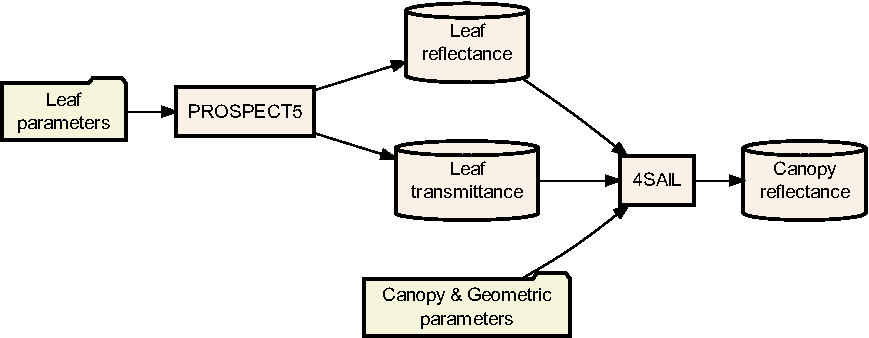
\includegraphics{_main_files/figure-latex/prosail-1.pdf}
\caption{\label{fig:prosail}Diagram of PROSAIL as a combination of PROSPECT5 and 4SAIL in the forward mode}
\end{figure}

\hypertarget{flim}{%
\section{Forest Light Interaction Model (FLIM)}\label{flim}}

The FLIM model was first developed by \citet{rosema1992new}, and it has stochastic properties. The FLIM model assumes that forests consist of discontinues mixture of gaps and crowns. In this model, canopy reflectance is considered to be a probability of seeing a gap (ground) or crown \citep{rosema1992new}. Table \ref{tab:flim} shows the input parameters of the FLIM model.

\begin{table}[H]

\caption{\label{tab:flim}Input parameters of FLIM}
\centering
\begin{tabu} to \linewidth {>{\raggedright\arraybackslash}p{8cm}>{\raggedright}X>{\raggedright}X}
\toprule
Parameter & Symbol & Unit\\
\midrule
Canopy reflectance at infinite depth & $R_{c}$ & $nm$\\
Background reflectance & $R_{g}$ & $nm$\\
Transmission in viewing direction & $T_{o}$ & $nm$\\
Transmission in sun direction & $T_{s}$ & $nm$\\
Stand density & SD & $ha^{-1}$\\
\addlinespace
Crown diameter & CD & $m$\\
Mean crown height & H & $m$\\
Solar zenith angle & tts & $^{\circ}$\\
Observer zenith angle & tto & $^{\circ}$\\
Sun-sensor azimuth angle & psi & $^{\circ}$\\
\bottomrule
\end{tabu}
\end{table}

The FLIM model assumes that the background reflectance (\(R_{g}\)) is known \citep{rosema1992new} and it is the reflectance coming from the forest floor \citep{atzberger2000development}. Transmission in viewing (\(T_{o}\)) and sun (\(T_{s}\)) direction parameters (Table \ref{tab:flim}) can be estimated using the SAIL model \citep{atzberger2000development, schlerf2006inversion}.

\hypertarget{inform}{%
\section{Invertable Forest Reflectance Model (INFORM)}\label{inform}}

The INFORM model was first developed by \citet{atzberger2000development}, and it consists of three sub-models. INFORM innovatively combines the three RTMs PROSPECT, SAIL and FLIM \citep{atzberger2000development, schlerf2006inversion}. The INFORM model can be used to efficiently simulate forest canopy bi-directional reflectance within the wavelength range of 400nm-2500nm \citep{schlerf2006inversion} and, compared to other 3D radiative transfer models, INFORM requires fewer input variables \citep{atzberger2000development, ali2020machine}.

The SAIL model can be used to calculate the parameters transmittance in the viewing (\(T_{o}\)) and sun (\(T_{s}\)) directions (Table \ref{tab:flim}) \citep{verhoef1984light}. However, in the SAIL model, the fact that the crown transmittance can be impacted (reduced) by woody parts of trees is ignored \citep{atzberger2000development}. Therefore, in the study by \citet{atzberger2000development}, it is shown that the INFORM model modifies the parameters transmittance in the viewing (\(T_{o}\)) and sun (\(T_{s}\)) direction in such a way that considers the shadow on the ground cast by woody parts of trees. However, in the study by \citet{schlerf2006inversion}, this technique was not applied because of the difficulties with parameterisation. Furthermore, INFORM represents leaf area index (LAI) as LAI of single trees (\(LAI_{s}\)) by dividing LAI by the canopy closure \citep{ali2016retrieval, ali2020machine}.

As the INFORM model is a combination of the three sub-models, its input parameters are simply the parameters of the sub-models. Therefore, the whole input parameters of the INFORM model can be found in Table \ref{tab:prospect5} (PROSPECT5), Table \ref{tab:4sail} (4SAIL) and Table \ref{tab:flim} (FLIM). Figure \ref{fig:inform} shows how INFORM can be used in the forward mode as a combination of PROSPECT5, 4SAIL and FLIM.

\begin{figure}
\centering
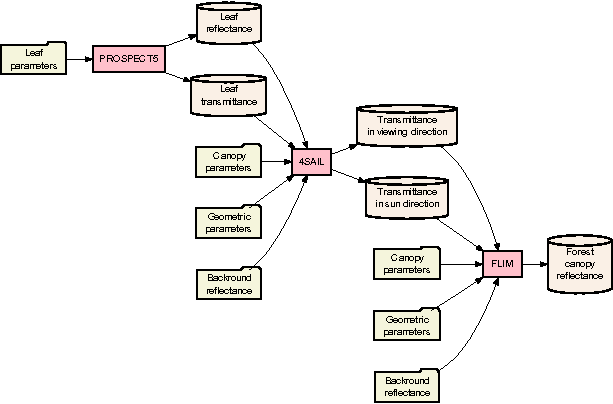
\includegraphics{_main_files/figure-latex/inform-1.pdf}
\caption{\label{fig:inform}Visualization of the INFORM model as a combination of PROSPECT5, 4SAIL and FLIM in the forward mode}
\end{figure}

Successful applications of the INFORM model to retrieve forest biophysical parameters from hyperspectral remote sensing satellite data have been confirmed by various studies. For example, in the studies by \citet{ali2016retrieval} and \citet{wang2017canopy}, the INFORM model was successfully used to retrieve forest biophysical maps from the hyperspectral airborne remote sensing data HySpex. INFORM's suitability to be applied for multispectral remote sensing data was also proved in different studies. For example, \citet{darvishzadeh2019mapping} used the INFORM RTM in order to retrieve forest leaf chlorophyll content content maps from the multispectral remote sensing satellite data Sentinel-2 and RapidEye. \citet{ali2020machine} also utilized the INFORM model to retrieve forest canopy plant traits from Sentinel-2 multispectral remote sensing data.

\hypertarget{chrtm}{%
\section{Challenges of RTMs}\label{chrtm}}

One of the main challenges of the RTMs is the so-called ill-posed problem \citep{combal2003retrieval, zhu2019estimation}. RTMs are mainly used for inversion problems. And inversion problems are usually ill-posed problems as opposed to well-posed problems. The ill-posed problem refers to a problem where multiple solutions can lead to similar or the same output. It makes the radiative transfer modelling process a very challenging process as multiple sets of solutions (e.g.~leaf/canopy variables) can yield very similar simulated reflectance to the measured reflectance \citep{combal2003retrieval, darvishzadeh2008estimation, zhu2019estimation}.

Fortunately, the problem of ill-posedness can be efficiently addressed using prior information \citep{combal2003retrieval, darvishzadeh2008estimation, zhu2019estimation}. \citet{combal2003retrieval} divides this prior information into three groups. The first category of prior information is to use data coming from the same spatial area but collected using another sensor (e.g.~radar). The second type of prior information is the knowledge about the architecture of the canopy that is being studied. This knowledge could help decide what type of RTM to select (turbid medium, geometric etc.). Finally, the last type of prior information to be considered is the knowledge of the usual distribution range of biophysical and biochemical variables of canopies. This information can be gained with the help of either specialist/expert knowledge or by combining experimental data \citep{combal2003retrieval}.

\hypertarget{mlra}{%
\chapter{Machine Learning Regression Algorithms (MLRA)}\label{mlra}}

Machine Learning Regression Algorithms (MLRA) are non-linear and non-parametric techniques that can be used to retrieve forest biophysical and biochemical parameters. Apart from non-parametric methods, there are also parametric techniques that can be used for the same purpose. However, the main advantage of the non-parametric methods over the parametric ones is the fact that they often do not assume any underlying relationships between the response (e.g.~plant traits) and predictor (e.g.~canopy reflectance) variables. These models do not rely on any linearity, which makes them very compelling techniques that can be applied in various research fields \citep{sinha2020estimation, rivera2015emulator, verrelst2019quantifying}.

According to the extensive review study by \citet{verrelst2019quantifying}, Decision Trees (DT), Kernel-Based Machine Learning Regression Methods (KBMLRM) and Artificial Neural Networks (ANN) are the three most widely used Machine Learning (ML) families for retrieval of plant biophysical and biochemical variables in remote sensing. This chapter focuses on the most commonly used ML techniques and briefly reviews them.

\hypertarget{dt}{%
\section{Decision Trees (DT)}\label{dt}}

Decision Tree (DT) methods rely on trees and branches to illustrate the outcome of each decision \citep{verrelst2019quantifying}. The Random Forest (RF) is a non-parametric learning model and it is also considered to be an ensemble model \citep{breiman2001random}. Essentially, the Random Forest Regression (RFR) algorithm builds multiple small regression trees where each tree has a vote on the prediction. Based on the votes of each tree, a final prediction is made \citep{breiman2001random, powell2010quantification}. The major advantage of the Random Forest model is that it is not sensitive to overfitting \citep{breiman2001random, powell2010quantification, verrelst2019quantifying}, which is a well-known phenomenon challenging many ML algorithms' performance. Apart from that, the RF algorithm can successfully deal with large amounts of training data as well as outliers and noise in the training data. These properties are the reason why the RF model is an attractive method for plant trait mapping applications in remote sensing \citep{verrelst2019quantifying}.

Essentially, there are two main parameters of the RF algorithm. These are the number of trees (ntree) and number of variables (mtry) that will be randomly sampled at every split \citep{wang2018estimation}. \citet{breiman2001random} suggests that a tree count of 500 (ntree = 500) may be sufficient in many cases.

The applicability of the RFR algorithm for retrieval of plant traits has been demonstrated in many studies. For example, \citet{ali2020machine} indicates that, when compared to the traditional Look Up Table (LUT) method with merit function, the RFR's retrieval accuracy was higher. In the studies by \citet{han2016hyperspectral} and \citet{pullanagari2016mapping}, RFR was compared to the other widely used ML algorithms (e.g.~SVM). In these studies, no method was found to be significantly superior to one another, indicating that all the widely used ML methods are highly competitive \citep{verrelst2019quantifying}.

\hypertarget{kernel}{%
\section{Kernel-Based Machine Learning Regression Methods (KBMLRM)}\label{kernel}}

Kernel-based learning algorithms rely on turning the current dimension of the data into a higher dimension and solving non-linear problems using a kernel function. Kernel methods offer very flexible implementation and they can be efficiently utilized as long as the linear problem can be solved in terms of dot products (linear algebra) \citep{verrelst2019quantifying}. According to the review study by \citet{gomez2011review}, kernel-based methods play a very important role in the remote sensing field. Kernel-based models can efficiently deal with small number of training samples (training data), very high-dimensional and noisy data sets. Unlike kernel-based algorithms, other machine learning methods, such as neural networks (NN), are known to be sensitive to the noise and high dimensions of the data, and importantly, they tend to perform very poorly when large training data sets are not available. All of these properties make kernel-based algorithms very attractive alternatives for remote sensing researchers as the mentioned issues that kernel-based algorithms handle are well-known for remote sensing data \citep{gomez2011review}.

Support Vector Regression (SVR) \citep{drucker1997support} is one of the most widely used KBMLRM \citep{verrelst2019quantifying}. One of the advantages of Support Vector Machines (SVM) (\citet{boser1992training}) over other ML methods such as ANN is that it mainly relies on minimizing the risk function, as opposed to trying to minimize the error in the training data set. Artificial neural networks, however, tries to minimize the error function, which makes them very susceptible to overfitting to the training data \citep{karimi2008application}. The applicability of SVM to estimate plant biophysical traits has been demonstrated in various studies. For example, \citet{karimi2008application} and \citet{yang2011estimating} used SVM to estimate plant biophysical parameters from hyperspectral remote sensing data. A study by \citet{tuia2011multioutput} demonstrated the successful use of multioutput SVR in order to retrieve the estimated biophysical parameters. Various studies compared the performance of SVR to the other ML methods. For example, \citet{pullanagari2016mapping} used different methods to map macro and micro nutrients from hyperspectral data. This study concluded that although SVR performed better for a certain parameter retrieval, this algorithm was not superior to the other ML methods in general.

Another widely used kernel-based ML method is Gaussian Process Regression (GPR). GPR is a Bayesian, non-parametric, and probabilistic ML method that provides important insights for retrieval of plant traits from remote sensing data \citep{camps2016survey, camps2019perspective}. The major advantage of GPR over the other widely used ML algorithms is that GP models provide confidence intervals for the estimations \citep{berger2020retrieval}. In other words, besides providing very good results, GPR can also give information about how much uncertainty (e.g.~error bars) exists in the predictions or estimations of the retrieved parameters. GPR can easily deal with different types of data and it can be implemented in a way that efficiently handles noise in the data. These issues commonly occur in remote sensing data, which makes the GPR algorithm very interesting for the remote sensing community \citep{camps2016survey, camps2019perspective}. Successful applications of GPR to retrieve plant biophysical and biochemical variables have been demonstrated in the literature. A relatively recent study by \citet{berger2020retrieval} used two versions of GPR (homoscedastic and heteroscedastic) for retrieval of plant nitrogen content. This study showed that the both versions of GPR performed well for the retrieval of plant nitrogen content. \citet{upreti2019comparison} used different ML methods to retrieve plant traits from the multispectral remote sensing satellite data Seninel-2. They found GPR to be the best performing algorithm within the cross-validation stage, but not in general \citep{upreti2019comparison}. A study by \citet{caicedo2014toward} compared different ML models in terms of accuracy and concluded that GPR yielded the most accurate results. However, it is important to note that GPR does not come without drawbacks. For example, one of the main challenges of GPR is that it is computationally costly despite advances \citep{camps2019perspective}.

\hypertarget{ann}{%
\section{Artificial Neural Networks (ANN)}\label{ann}}

Artificial Neural Networks (ANN) is a powerful ML method that consists of neurons and layers \citep{simon1999neural}. Usually, the ANN has three main components: an input layer, (a) hidden layer(s) and an output layer \citep{jensen1999predictive, quan2017radiative}. A typical mechanism for training an ANN is that first a training data set is given to the model as an input layer and then, the model trains and predicts output. Once the predicted output is available, the current predicted output is compared to the true output so that the weight parameters can be adjusted in a way that the predicted and true output are closely similar \citep{ingram2005mapping, quan2017radiative}. This learning process can be repeated multiple times until similarity between the predicted and true outputs is at a certain threshold (e.g.~convergence). This threshold can be defined by the user depending on their preferences \citep{jensen1999predictive, quan2017radiative}.

Main advantages of ANN are their simplicity, computational efficiency and their ability to learn from data where linearity is not assumed \citep{schlerf2006inversion, walczak2019artificial}. Furthermore, ANNs do not require any prior information about the distribution that the data come from unlike the traditional statistical methods \citep{walczak2019artificial}.

ANNs have been utilized in the remote sensing domain, especially for plant property mapping, since the 1990s \citep{verrelst2019quantifying}. There are many studies in the literature that show the superiority of the ANN methods to more traditional statistical methods. For example, studies by \citet{malenovsky2013retrieval} and \citet{kalacska2015estimation} showed that compared to the traditional statistical and vegetation index (VI) methods, ANN yielded more accurate results for retrieval of plant parameters from hyperspectral remote sensing data. \citet{neinavaz2016retrieval} compared ANN's performance to other methods (e.g.~linear parametric) and found that ANN was superior to the compared methods for retrieval of an important plant variable, LAI. Moreover, a recent study by \citet{danner2021efficient} used four widely used ML methods to retrieve plant traits and compared the results of each method. In general, ANN was found to be the best performing ML method among the others, considering the models' efficiency, robustness, accuracy, and computational time.

Despite being a powerful ML method, ANN comes with drawbacks. There are many descriptors in a typical ANN that may be correlated to each other. Because of that, there is a risk of the model being stuck in the local minima. Another well-known challenge of ANN is that it is susceptible to overfitting. Fortunately, there have been many methods developed to deal with these problems (e.g.~regularization) \citep{ghasemi2018neural}. A study by \citet{schlerf2006inversion} points out another potential drawback, which is the fact that the ANN model may behave unpredictably when the model does not represent the spectral properties of the target variable well.

\hypertarget{chml}{%
\section{Challenges of Machine Learning Regression Algorithms (MLRA)}\label{chml}}

There are common issues that almost all MLRAs are challenged with. Hyperspectral remote sensing data come with many bands that may be highly correlated and noisy. This problem is a well-known problem and it is also called the ``Hughes phenomenon'' \citep{hughes1968mean} or the ``curse of dimensionality'' \citep{danner2021efficient}. One of the main problems is that MLRAs' computational cost becomes higher with an increased amount of training data. Most MLRAs require high computational power for very costly training phases. Apart from that, many highly correlated bands may indicate highly redundant data which cause difficulties for statistical and ML methods \citep{rivera2017hyperspectral}.

There are some methods that can be used to efficiently deal with the ``curse of dimensionality'' problem. Some of the most commonly used methods for dealing with this issue involve reducing the space (dimension) of the original data. \citet{rivera2017hyperspectral} indicate that this issue can be solved in two different domains. The first method involves choosing the samples that provide most of the information compared to the other samples. The second domain involves the use of feature selection or dimensionality reduction (DR) techniques. In the first technique, the amount of samples is minimized but accuracy is still a priority \citep{rivera2017hyperspectral}.

The second set of techniques (DR) tries to reduce the original data space while keeping most of the information available. In other words, DR techniques convert a large number of features with a high amount of redundancy into a much smaller feature set with no or as little redundancy as possible \citep{lee2007nonlinear}. Two of the commonly used DR techniques to compress the spectral reflectance data in remote sensing are so-called wavelet transform (WT) and principal component analysis (PCA) \citep{ke2016estimating}.

After reducing the dimension of the original data, new and low-dimensional data can be used to train ML models. MLRAs can be combined with PCA to reduce the computational cost and avoid the ``curse of dimensionality'' problem. There have been studies comparing the performance of ML methods when combined with DR techniques to feature selection or VI based ML applications. For example, \citet{liu2017hyperspectral} compared the performance of PCA based ANN with VI based ANN and concluded that using PCA before training is superior to using VI in the training phase. However, it is also important to note that PCA is not the only DR technique, although it is the most commonly used DR technique in plant retrieval studies by remote sensing researchers. A study by \citet{rivera2017hyperspectral} reviews and compares different DR techniques and concludes that PCA is not always the best performing DR technique and the use of other techniques may yield better results in some cases.

In general, most ML algorithms need a large amount of training data to learn from the training data and generalize well to the data that were not used in the training phase (e.g.~test data). This leads to another challenging property of ML for retrieval of plant biophysical traits. This is because of the fact that it is extremely difficult to collect enough training data for plant traits in the field for a ML method to perform well. It requires various \emph{in-situ} field techniques and these techniques need to be used in a limited time-frame. It is still not guaranteed that training data collected in the field can generalize well to other fields \citep{danner2021efficient}. One way to overcome this problem is to use the so-called hybrid-machine learning method.

\hypertarget{hml}{%
\chapter{Hybrid Machine Learning Method}\label{hml}}

The hybrid machine learning method is a combination of physically based RTMs and MLRAs. The main idea behind this technique is to make use of the advantages of the two different methods at the same time. RTMs can provide simulated data based on well-known and approved physical laws. Therefore, the data provided by RTMs can be applicable universally. Machine learning methods provide opportunities to efficiently deal with non-linear data (without making assumptions) in a reasonable time frame \citep{abdelbaki2021comparison, de2020quantifying, berger2021survey, ke2016estimating}. The study by \citet{fernandez2021hybrid} mentions three main advantages of using the hybrid method over other techniques: better generalization of the model, better estimation of the biophysical parameters, and finally, more efficient computation.

A typical procedure for using hybrid machine learning methods to retrieve plant biophysical variables involves simulating coupled leaf and canopy models (e.g.~PROSAIL) and storing the simulated data in the so-called look-up-table (LUT). The LUT typically stores simulated reflectance data and a wide range of plant parameters. Once the LUT is available, a ML model can be trained using all the information available in the LUT as a training data set \citep{verrelst2019quantifying}.

There have been a large number of studies utilizing hybrid machine learning methods for retrieval of plant traits. For example, a recent study by \citet{cesar2021exploring} combines PROSAIL and widely used MLRAs with the hybrid approach in order to retrieve plant parameters from Sentinel-2 satellite data. In this study, the performance of each MLRA combined with PROSAIL was assessed when noise was added. In the study by \citet{wei2017estimation}, plant LAI was successfully estimated using random forest regression and PROSAIL in a hybrid work flow. \citet{verrelst2016active} used hybrid RTM and kernel-based machine learning techniques to estimate plant leaf area index and chlorophyll content. This study included the active learning (AL) technique for an efficient retrieval strategy.

\hypertarget{satellite-data}{%
\chapter{Satellite Data}\label{satellite-data}}

In this study, the hyperspectral satellite data PRISMA (PRecursore IperSpettrale della Missione Applicativa) was utilized. The PRISMA sensor has Field of View (FOV) of \(2.45^{\circ}\) and swath of 30 km. The sensor takes images within the spectral range of 400-2500nm. The PRISMA image has 66 bands in the visible and near infrared (VNIR) region (400-1010nm) and 173 bands within the short-wave infrared (SWIR) region (920-2505nm) of the spectrum. The spectral resolution of the data is somewhere between 6nm and 12nm. The hyperspectral data has a ground sampling distance (GSD) of 30 m \citep{candela2016prisma, giardino2020first, verrelst2021mapping}. The scientific fields that are expected to largely benefit from the PRISMA data are mainly environmental, climate change and forest research areas, among others \citep{giardino2020first}.

In this study, L2 product of PRISMA data was retrieved and processed. First, the image was cropped to the study area using a polygon shape file covering the study area. Only 231 bands of the PRISMA image were available and all the available bands were utilized for further analysis. The PRISMA image contained clouds and shadow within the national park area and therefore, pre-processing of the image was necessary. The software package ENVI was used in order to accurately mask out the shadows and clouds available within the study area.

\hypertarget{study-area}{%
\chapter{Study area}\label{study-area}}

Hunsrück-Hochwald is a German national park that was founded in 2015. The national park covers areas in both Saarland and Rhineland-Palatinate German federal states (Figure \ref{fig:germanmap}).

\begin{figure}
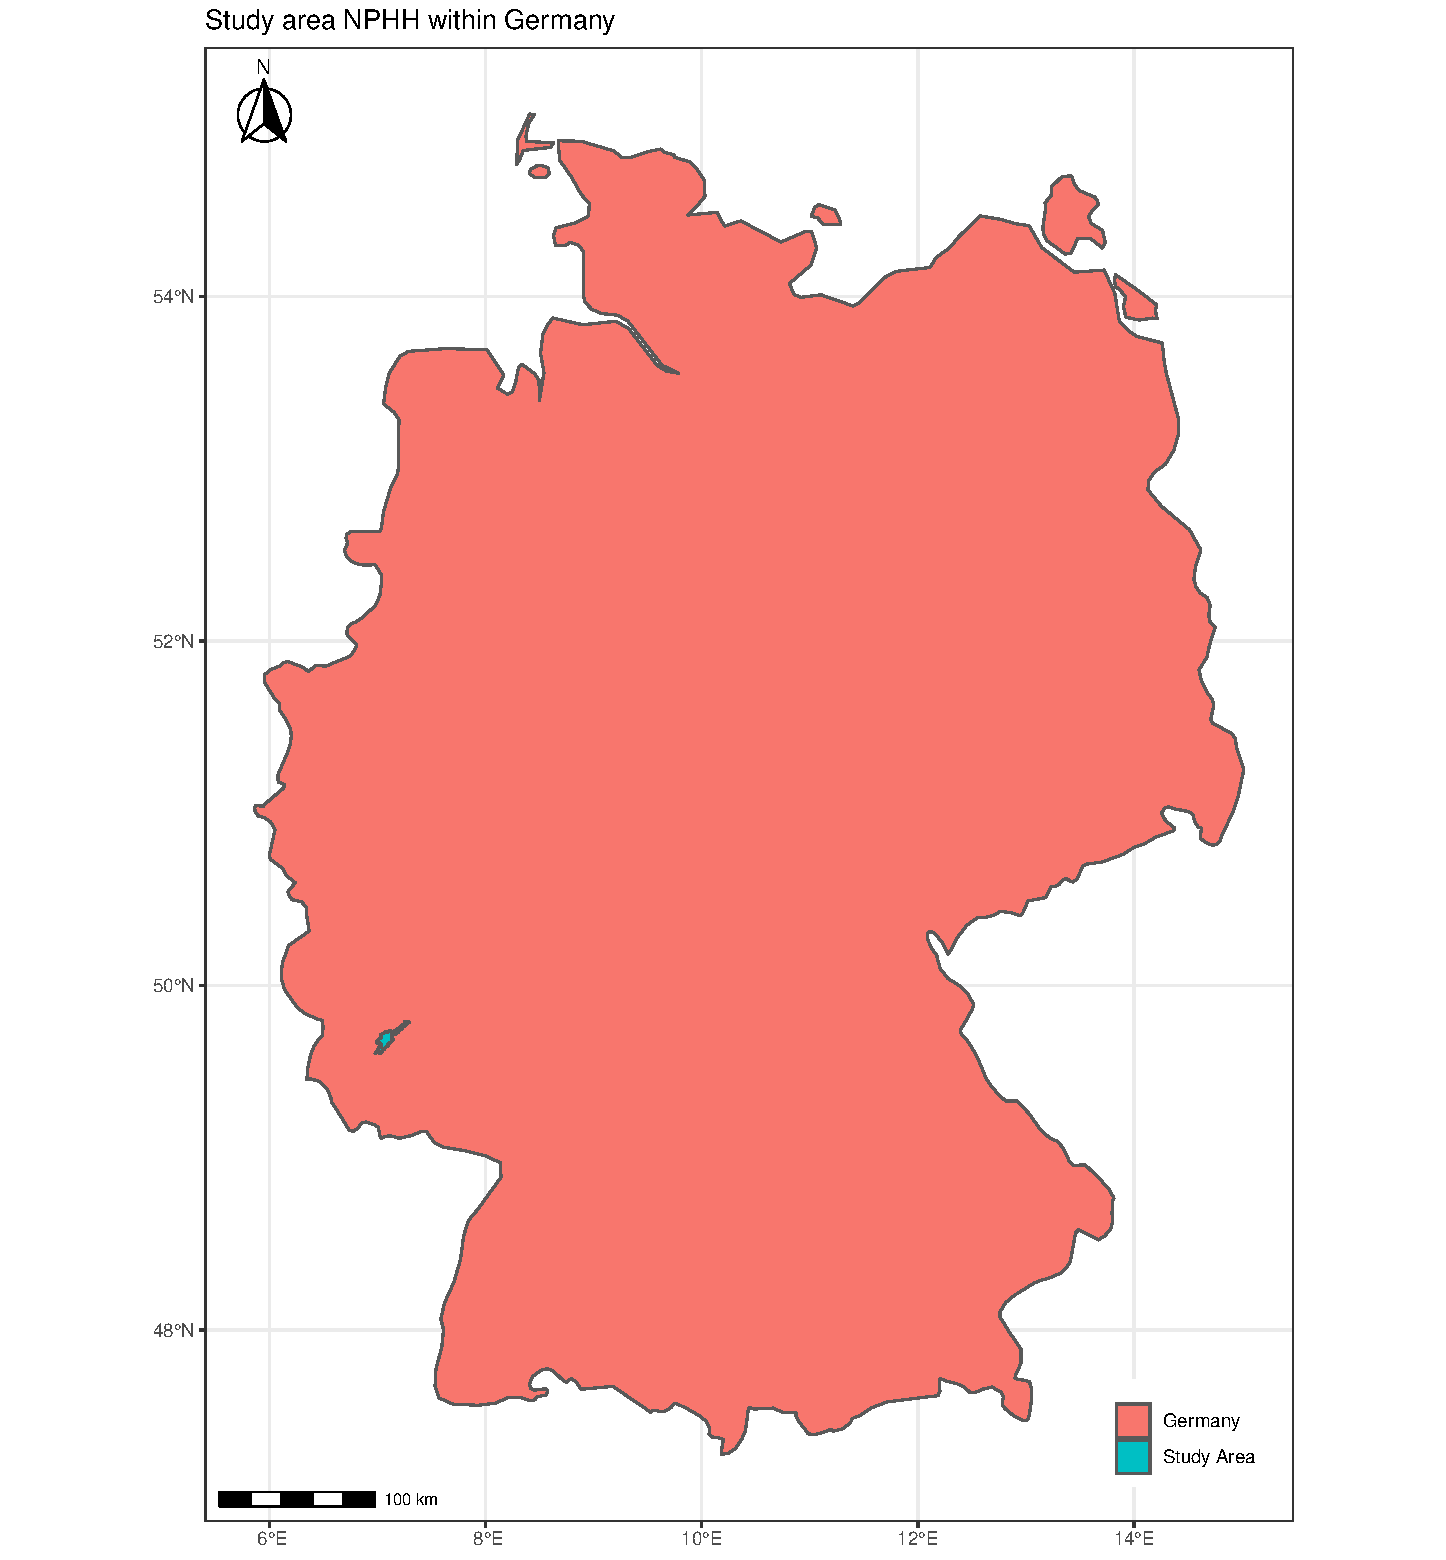
\includegraphics[width=0.9\linewidth]{./figures/map_germany} \caption{The study area on Germany's map.}\label{fig:germanmap}
\end{figure}

The area of the national park is about 10,000 hectare \citep{fischer2016scientific}. There are various forestry activities (selective cutting etc.) occuring in the national park area. The forest is mainly dominated by the plant species Norway spruce (\emph{Picea abies}), oak (\emph{Quercus petraea}) and beech (\emph{Fagus sylvatica}) \citep{buddenbaum2015nationalpark}.

\begin{figure}
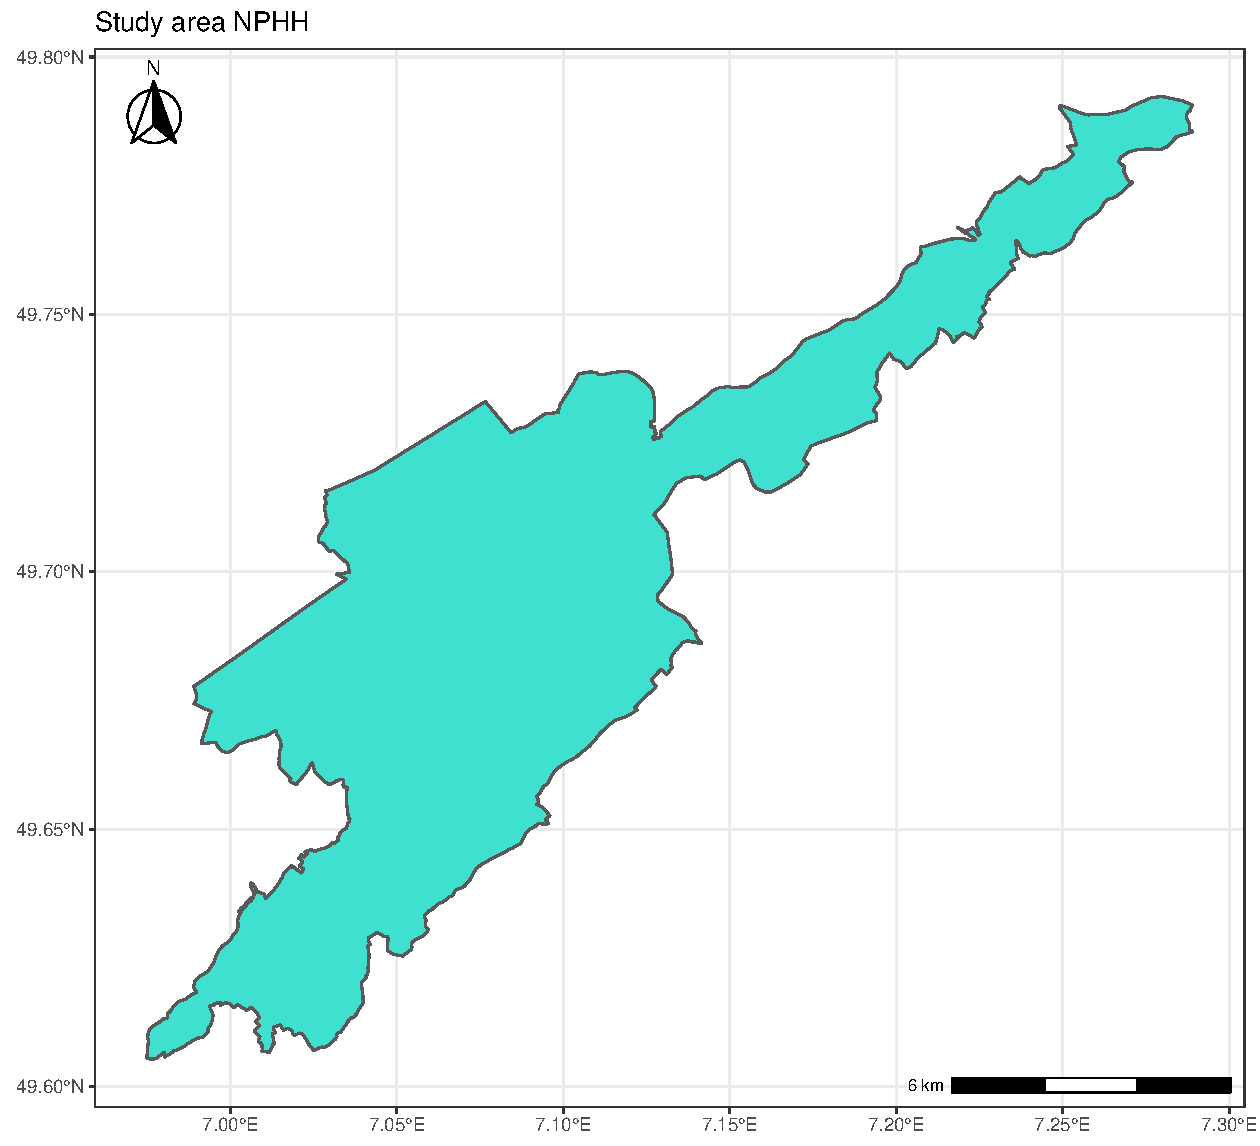
\includegraphics[width=0.9\linewidth]{./figures/map_np} \caption{The study area.}\label{fig:npmap}
\end{figure}

\hypertarget{methods}{%
\chapter{Methods}\label{methods}}

This section explains the methods used in this research.

\hypertarget{local-sensitivity-analysis}{%
\section{Local sensitivity analysis}\label{local-sensitivity-analysis}}

Local sensitivity analysis was performed to assess the effect of each of the main 6 plant biochemical and biophysical variables on the PRISMA image bands. In the local sensitivity analysis, simulation is performed by keeping all the variables constant at their determined or default values except the parameter of interest. This way the effect of a specific parameter on the simulated spectra can be assessed. In this research the plant parameters \(C_{ab}\), \(C_{w}\), \(C_{m}\), \(LAI_{s}\), \(CD\) and \(SD\) were varied each 15 times (Table \ref{tab:tsvaried}), while keeping the rest of the variables at their default values (Table \ref{tab:tsfixed}). The default and varied values were chosen based on the available studies in the literature (e.g. \citet{darvishzadeh2019mapping}; \citet{laurent2011inversion}; \citet{schlerf2012vegetation}) where similar RTM method was used to simulate reflectance for Spruce trees.

Table \ref{tab:tsvaried} shows the 6 parameters that were varied, their units, minimum and maximum values. Each parameter was varied 15 times, meaning 15 different spectra were simulated for each variable.

\begin{table}[H]

\caption{\label{tab:tsvaried}INFORM parameters varied in local sensitivity analysis (each parameter were varied 15 times)}
\centering
\begin{tabu} to \linewidth {>{\raggedright\arraybackslash}p{8cm}>{\raggedright}X>{\raggedright}X>{\raggedright}X>{\raggedright}X}
\toprule
Parameter & Abbrev. & Unit & Min & Max\\
\midrule
Chlorophyll content & $C_{ab}$ & $\frac{\mu g}{cm^2}$ & 20 & 60\\
Equivalent water thickness & $C_{w}$ & $\frac{g}{cm^2}$ & 0.0035 & 0.035\\
Leaf dry matter content & $C_{m}$ & $\frac{g}{cm^2}$ & 0.008 & 0.03\\
Leaf area index (single) & $LAI_{s}$ & $\frac{m^2}{m^2}$ & 0 & 7\\
Stem density & $SD$ & $ha^{-1}$ & 200 & 5000\\
\addlinespace
Crown diameter & $CD$ & $m$ & 1.5 & 8.5\\
\bottomrule
\end{tabu}
\end{table}

\newpage

Table \ref{tab:tsfixed} shows the determined default values for each INFORM parameter that were kept during the sensitivity simulation while one of the parameter was varied (Table \ref{tab:tsvaried}).

\begin{table}[H]

\caption{\label{tab:tsfixed}INFORM Parameters that were kept constant while one parameter was varied at a time}
\centering
\begin{tabu} to \linewidth {>{\raggedright\arraybackslash}p{8cm}>{\raggedright}X>{\raggedright}X>{\raggedright}X}
\toprule
Parameter & Abbr & Unit & Value\\
\midrule
Leaf structure parameter & $N$ & $-$ & 3\\
Chlorophyll content & $C_{ab}$ & $\frac{\mu g}{cm^2}$ & 40\\
Leaf cartenoid content & $C_{ar}$ & $\frac{\mu g}{cm^2}$ & 8\\
Brown Pigment Content & $C_{brown}$ & $-$ & 0.001\\
Equivalent water thickness & $C_{w}$ & $\frac{g}{cm^2}$ & 0.0117\\
\addlinespace
Leaf dry matter content & $C_{m}$ & $\frac{g}{cm^2}$ & 0.03\\
Average leaf inclination angle & $ALIA$ & $^{\circ}$ & 65\\
Leaf area index (single) & $LAI_{s}$ & $\frac{m^2}{m^2}$ & 6\\
Leaf area index (understorey) & $LAI_{u}$ & $\frac{m^2}{m^2}$ & 0.5\\
Hot spot parameter & $Hot$ & $\frac{m}{m}$ & 0.02\\
\addlinespace
Solar zenith angle & $tts$ & $^{\circ}$ & 45.43\\
Observer zenith angle & $tto$ & $^{\circ}$ & 0\\
Sun-sensor azimuth angle & $psi$ & $^{\circ}$ & 181.41\\
Soil brightness & $\alpha_{soil}$ & $-$ & 0.5\\
Stem density & $SD$ & $ha^{-1}$ & 700\\
\addlinespace
Crown diameter & $CD$ & $m$ & 5\\
Mean Height & $H$ & $m$ & 20\\
Fraction of diffuse incoming & $skyl$ & $-$ & 0.1\\
Soil reflectance spectrum & $B_{g}$ & $-$ & default\\
\bottomrule
\end{tabu}
\end{table}

\emph{Solar zenith angle} and \emph{Sun-sensor azimuth angle} were calculated based on the PRISMA image acquisition parameters (date, lat/long etc.) using the \emph{solar position calculator} at \url{https://www.esrl.noaa.gov/gmd/grad/solcalc/azel.html}.

RTM models PROSPECT5, 4SAIL and FLIM were coupled (INFORM) in order to simulate canopy reflectance. Simulations were carried out using the \emph{ccrtm} package \citep{ccrtm} in \emph{R} \citep{r}. The default soil spectra provided by the the \emph{ccrtm} package \citep{ccrtm} was used for the simulations. Spectral resampling was performed in order to resample the INFORM output spectra (1nm resolution between 400nm and 2500nm) into PRISMA image bands. For spectral resampling the \emph{R} package \emph{hsdar} \citep{hsdar} was utilized.

\hypertarget{rtm-simulation-inform}{%
\section{RTM simulation (INFORM)}\label{rtm-simulation-inform}}

PROSPECT5, 4SAIL and FLIM RTM models were coupled (INFORM) to simulate forest canopy reflectance based on different values of plant biophysical and biochemical parameters. The 6 parameters that were mentioned in the previous chapter were varied and spectra was simulated based on each combination of these variables. The number of combinations increase exponentially, which in turn requires increased computational power. Therefore, the trade-off must be taken into account between computational power or time and accurate simulation.

Different authors suggest different number of LUT size for RTM simulation. For example, \citet{danner2021efficient} mention that LUT size of minimum 50,000 is recommended. \citet{ali2020machine} and \citet{darvishzadeh2019mapping} created a LUT size of 100,000 and 500,000 respectively.

In this research, LUT size of 316,800 was created based on each combination of different plant biophysical and biochemical parameters. The range of the varied parameters and parameters that were kept constant were determined based on the suggestions of the studies that were mentioned in the previous chapter. These studies used similar methods to simulate canopy reflectance for mainly Spruce forests/trees.

Table \ref{tab:tinformfull} shows the variables that were used to simulate forest canopy parameters. Table \ref{tab:tinformfull} also contains information about the range of the values and how many times each parameter was varied.

\newpage

\begin{table}[H]

\caption{\label{tab:tinformfull}Range of full input parameters that were used to create a LUT size of 316800}
\centering
\begin{tabu} to \linewidth {>{\raggedright\arraybackslash}p{8cm}>{\raggedright}X>{\raggedright}X>{\raggedright}X>{\raggedright}X>{\raggedright}X}
\toprule
Parameter & Abbr & Unit & Min & Max & Steps\\
\midrule
Leaf structure parameter & $N$ & $-$ & 3 & 3 & $-$\\
Chlorophyll content & $C_{ab}$ & $\frac{\mu g}{cm^2}$ & 20 & 60 & 15\\
Leaf cartenoid content & $C_{ar}$ & $\frac{\mu g}{cm^2}$ & 8 & 8 & $-$\\
Brown Pigment Content & $C_{brown}$ & $-$ & 0.001 & 0.001 & $-$\\
Equivalent water thickness & $C_{w}$ & $\frac{g}{cm^2}$ & 0.0035 & 0.035 & 10\\
\addlinespace
Leaf dry matter content & $C_{m}$ & $\frac{g}{cm^2}$ & 0.008 & 0.03 & 11\\
Average leaf inclination angle & $ALIA$ & $^{\circ}$ & 65 & 65 & $-$\\
Leaf area index (single) & $LAI_{s}$ & $\frac{m^2}{m^2}$ & 0 & 6.5 & 16\\
Leaf area index (understorey) & $LAI_{u}$ & $\frac{m^2}{m^2}$ & 0.5 & 0.5 & $-$\\
Hot spot parameter & $Hot$ & $\frac{m}{m}$ & 0.02 & 0.02 & $-$\\
\addlinespace
Solar zenith angle & $tts$ & $^{\circ}$ & 45.43 & 45.43 & $-$\\
Observer zenith angle & $tto$ & $^{\circ}$ & 0 & 0 & $-$\\
Sun-sensor azimuth angle & $psi$ & $^{\circ}$ & 181.41 & 181.41 & $-$\\
Soil brightness & $\alpha_{soil}$ & $-$ & 0.5 & 0.5 & $-$\\
Stem density & $SD$ & $ha^{-1}$ & 200 & 5000 & 4\\
\addlinespace
Crown diameter & $CD$ & $m$ & 1.5 & 8.5 & 3\\
Mean Height & $H$ & $m$ & 20 & 20 & $-$\\
Fraction of diffuse radiation & $skyl$ & $-$ & 0.1 & 0.1 & $-$\\
Soil reflectance spectrum & $B_{g}$ & $-$ & default & default & $-$\\
\bottomrule
\end{tabu}
\end{table}

All simulations were performed using the library \emph{ccrtm} \citep{ccrtm} in \emph{R} programming language \citep{r} using the most recent version 4.1.0. Generating a LUT size of 316,800 is an expensive process from a computational standpoint (depending on how much computer resources and time are available this might change). Also, all simulations are independent of each other, meaning simulation of one spectra has no effect on the other, as every simulated spectra is simulated based on a different combination of parameters. These two factors make the generation of such a large LUT good candidate for parallel computation. Therefore, the software packages \emph{doParallel} \citep{doparallel} and \emph{foreach} \citep{foreach} were utilized for parallel computation (using all the available cores) in \emph{R} programming language \citep{r}. This significantly reduced the computational time. All of the simulations were computed on a Lenovo Thinkpad E480 running under Windows 10 operating system with a processor Intel(R) Core(TM) i7-8550U CPU @ 1.80GHz, 2001 Mhz, 4 Core(s), 8 logical processor(s).

\hypertarget{spectral-resampling}{%
\section{Spectral resampling}\label{spectral-resampling}}

The output of INFORM simulations have 1nm spectral resolution within the range of 400nm-2500nm and needs to be spectrally resampled to PRISMA image bands. In this research, the spectral response function of the PRISMA image was used. Band center wavelengths and full width half maximum values were extracted from the PRISMA image metadata and used for spectral resampling. For spectral resampling, the \emph{R} package \emph{hsdar} \citep{hsdar} was utilized.

\hypertarget{statistics-of-simulated-data-and-prisma-image}{%
\section{Statistics of simulated data and PRISMA image}\label{statistics-of-simulated-data-and-prisma-image}}

Statistical information such as standard deviation and mean were calculated for the simulated (and resampled to PRISMA bands) data and all the pixels of the PRISMA image within the study area. Pixels that are out of the study area boundary were masked out. Then, average spectra in the LUT (synthetic database) and PRISMA image (only study area) were compared to each other. LUT contains 316,800 simulated spectra, the number of pixels within the study area in the PRISMA image is only 95,517. Statistical information were extracted using the libraries in the \emph{tidyverse} package \citep{tidyverse} and the plots for visualization were produced using \emph{ggplot2} \citep{ggplot2}.

\hypertarget{gaussian-noise}{%
\section{Gaussian noise}\label{gaussian-noise}}

Simulated reflectance data usually do not contain any noise. This is, however, not the case with remote sensing data as they are commonly found to contain various types of noise \citep{rivera2017hyperspectral}. In this study, 3\% Gaussian noise was added to each simulated spectra in the LUT in order to make the simulated data more similar to the real remote sensing data. In order to assess the effect of adding 3\% Gaussian noise to the simulated data, one spectra from the LUT and one pixel from the PRISMA image were randomly picked and plotted.

\hypertarget{defining-training-validation-and-testing-sets}{%
\section{Defining training, validation and testing sets}\label{defining-training-validation-and-testing-sets}}

The data in the LUT was divided into training, validation and testing sets. Model building and training will be done using only the training set. Validation set will be used to validate the model (e.g.~assessing the impact of different hyper-parameters) and the performance of the final model will be tested using the testing set. This step is important because it will allow us to monitor whether the model can generalize to the data (e.g.~testing set) it was not trained on.

First, the full data set was shuffled and about 20\% of the data was randomly sampled and assigned to validation and testing sets (10\% validation, 10\% testing sets). Random sampling ensures that there is no any pattern contained in any of the divided data sets.

\hypertarget{data-processing}{%
\section{Data processing}\label{data-processing}}

First, the simulated canopy reflectance in the training data set was normalized and standardized using the Equation \eqref{eq:norm}:

\begin{equation}
Band_{n_{scaled}}\ =\ \frac{Band_n\ -\ \mu_{Band_n}}{\sigma_{Band_n}}
\label{eq:norm}
\end{equation}

Here \(Band_{n}\) refers to the reflectance values in the \(n\)th simulated band and \(\mu_{Band_n}\) and \(\sigma_{Band_n}\) are mean and standard deviation of the reflectance values in the \(n\)th simulated band. \(Band_{n_{scaled}}\) is a transformed version of \(Band_{n}\) that has a mean of 0 and standard deviation of 1. This step ensures that all simulated bands have the same mean and standard deviation.

Data normalization and standardization were only performed using training data set. Mean and standard deviation of the training set were then used to transform the validation and testing data sets.

\hypertarget{principal-component-analysis-pca}{%
\section{Principal Component Analysis (PCA)}\label{principal-component-analysis-pca}}

Hyperspectral remote sensing data can contain many highly correlated bands. Dimensionality reduction techniques can be efficiently used to reduce the dimensions of hyperspectral remote sensing data. Benefits of reducing the dimensions of simulated data in plant biophysical variable retrieval studies have been demonstrated \citep{danner2021efficient, rivera2017hyperspectral}. In this study, one of the most commonly used DR technique Principal Component Analysis (PCA) was performed. In general, PCA tries to capture as much variation as possible with smaller number variables compared to the original data. PCA produces new variables called Principal Components and each Principal Component (PC) contains certain amount of variation available in the original data. Typically first PC contains the most variation, the second PC contains the second most variation and so on \citep{bro2014principal}.

Like in the processing step, PCA was only applied to the training data and the PCA result in the training data was used to transform the validation and testing sets. Cumulative sum of the variations the PCs contain was calculated in order to assess the proportion of the variation that can be explained with fewer variables than the original data (LUT). PCA and data processing performed using the package \emph{recipes} \citep{recipes} in \emph{tidymodels} \citep{tidymodels}.

\hypertarget{artificial-neural-networks-ann}{%
\section{Artificial Neural Networks (ANN)}\label{artificial-neural-networks-ann}}

Considering the fact that we have relatively large number of training examples, non-linear relationship between the input variables (image bands or PCs) and target variables (biophysical and biochemical variables), many different modern and optimization algorithms developed that can learn various types of non-linear relationships, and finally availability of the optimized open source software packages and support, Artificial Neural Network was chosen as a training model in this study.

Deep Neural Networks (DNN) is a specialized name for Artificial Neural Networks. DNN are also called Deep Feedforward Networks. Feedfoward network algorithm refers to an algorithm that tries to use the input example data \(x\) to learn a function \(f()\) that approximates the output variable \(y\) by adjusting the weights variable \(\theta\) \citep{goodfellow2016deep}:

\begin{equation}
y\ =\ f\left(x;\ \theta\right)
\label{eq:feed}
\end{equation}

These algorithms are called networks due to the fact that they usually consist of multiple functions connected to each other with networks. Neural Networks are typically composed of multiple layers, such as input, hidden and output layers. Input layer is typically the training examples and output layer is the target variable (e.g.~variable to predict). Hidden layers are in between input and output layers and different functions can be applied to different hidden layers \citep{goodfellow2016deep}. For example, the Equation \eqref{eq:dnn} shows a function \(f(x)\) that is formed by three hidden layers:

\begin{equation}
f\left(x\right)\ =\ f^{\left(3\right)}\left(f^{\left(2\right)}\left(f^{\left(1\right)}\left(x\right)\right)\right)
\label{eq:dnn}
\end{equation}

In the Equation \eqref{eq:dnn}, \(f^{(1)}\), \(f^{(2)}\) and \(f^{(3)}\) are the first, second and third layers, respectively. During the learning process, the neural network model is shown the output variables \(y\) of corresponding input variables \(x\) and the job of the hidden layers is to figure out how to match the target variable \(y\) as closely as possible \citep{goodfellow2016deep}.

In this research, two neural network models were built. The first model was trained using only 5 PCs as input variables, and the second neural network was trained using simulated 231 PRISMA bands. The aim of building two neural network models is to compare the performance of a neural network using only 5 PCs to a neural network that uses the original 231 simulated PRISMA bands to predict the output variables. This could help assess whether ANN can deal with the multi-collinearity that is available in hyperspectral remote sensing data.

\hypertarget{cost-function}{%
\subsection{Cost function}\label{cost-function}}

Choosing an appropriate cost function is an important part of building neural networks model. Essentially, cost function is what the neural network tries to minimize after each iteration. The cost function mean squared error (MSE) is the most widely used cost function for neural network models when the target variable is continuous \citep{allaire2018deep}.

In this study, MSE was chosen to be the cost function of the neural network models. The Equation \eqref{eq:mse} shows how the cost function MSE is defined:

\begin{equation}
MSE\ =\ \frac{1}{N}\sum_{i\ =\ 1}^n\left(y_i\ -\ f\left(x_i;\ \theta\right)\right)^2
\label{eq:mse}
\end{equation}

In the Equation \eqref{eq:mse}, \(N\) is the number of examples, \(y_{i}\) is the \(i\)th true value and \(f(x_{i}; \theta)\) is the predicted \(i\)th value. \(x_{i}\) refers to the input parameter of \(i\)th example, and \(\theta\) typically refers to weight term \(w\) and a bias term \(b\).

Apart from MSE, mean absolute error (MAE) was calculated as a metric and monitored during the training. MAE is defined as shown in the Equation \eqref{eq:mae}:

\begin{equation}
MAE\ =\ \frac{1}{N}\sum_{i\ =\ 1}^n\left|y_i\ -\ f\left(x_i;\ \theta\right)\right|
\label{eq:mae}
\end{equation}

\hypertarget{optimizer-algorithm}{%
\subsection{Optimizer algorithm}\label{optimizer-algorithm}}

In this research, Adam optimizer \citep{kingma2014adam} was applied to the neural network model. Before explaining what Adam does, it is important to visit the Stochastic gradient descent (SGD) algorithm.

Stochastic gradient descent is a very important algorithm used to build neural network models. SGD is used to update the learned weight and bias parameters \(\theta\). Let's assume that we have a model that tries to minimize the cost function \(J(\theta)\)

\begin{equation}
J\left(\theta\right)\ =\ \frac{1}{m}\sum_{i\ =\ 1}^mL\left(x^i,\ y^i,\ \theta\right)
\label{eq:cs}
\end{equation}

where L is the amount of loss for the \(i\)th example. Then, we compute the gradient as shown in the Equation \eqref{eq:derivative}:

\begin{equation}
\nabla_{\theta}J\left(\theta\right)\ =\ \frac{1}{m}\sum_{i\ =\ 1}^m\nabla_{\theta}L\left(x^i,\ y^i,\ \theta\right)
\label{eq:derivative}
\end{equation}

Finally, we can update the weight and bias parameters within the term \(\theta\):

\begin{equation}
\theta\ \leftarrow\ \theta\ -\ \epsilon\\\nabla_{\theta}J\left(\theta\right)\
\label{eq:gd}
\end{equation}

In the Equation \eqref{eq:gd} \(\epsilon\) is called learning rate and needs to be tuned. The learning rate parameter \(\epsilon\) is a very important hyperparameter for neural network and it is considered to be the most difficult hyperparameter to tune \citep{goodfellow2016deep}. Batch gradient descent uses the same idea, but unlike SGD, batch gradient descent makes an update for the whole training set after each iteration \citep{ruder2016overview}.

Usually, some of the directions in the parameter space can have a significant effect on the cost and some of them may not have any effect at all. Adaptive learning algorithms can efficiently solve this problem. One of the most commonly used adaptive learning algorithm is Adam \citep{kingma2014adam}. Essentially, Adam can be thought as a combination of RMSProp \citep{hinton2012neural} and Momentum \citep{polyak1964some} algorithms with minor differences. In the RMSProp algorithm, exponentially decaying averages are used to mitigate the problem of extreme updates. This helps the model converge more rapidly and less sensitive to extreme cases. The Momentum algorithm uses additional parameter called velocity \(v\) apart from learning rate \(\epsilon\). And during the gradient descent update, the velocity term \(v\) is additionally taken into consideration. The Adam algorithm implements first and second order moment terms. Unlike RMSProp, Adam also implements correction for the bias of first and second order moments \citep{goodfellow2016deep}. \citet{goodfellow2016deep} can be referred to for more detailed explanation of how the algorithms RMSProp, Momentum and Adam are implemented.

The main drawback of Adam is that now there are more hyperparameters to tune compared to simpler algorithms such as SGD. The Adam optimizer requires the hyperparameters step size \(\epsilon\), exponential decay rates \(p1\) and \(p2\) and a constant \(\delta\). In this study, the suggested default value of 0.001 was used for the step size term \(\epsilon\). \(p1\) and \(p2\) were set to 0.9 and 0.999 respectively (suggested values). The constant term \(\delta\) is \(10^{-8}\). Different most commonly used learning rate values (\(lr\)) were tested. The optimum learning rate value (specific to this study) was found to be 0.0001.

\hypertarget{mini-batch-size}{%
\subsection{Mini batch size}\label{mini-batch-size}}

Performing gradient update for the whole training set after each iteration can cause the computational cost to increase rapidly when the training data size \(m\) is large. Mini batch gradient descent can efficiently overcome this problem \citep{goodfellow2016deep}. Mini batch gradient descent makes updates for the mini batch size of \(n\), as opposed to updating gradients after training on the whole training data, with a size of \(m\) \citep{ruder2016overview}.

Considering the fact that our training data is relatively large (\(m = 250,120\)), we implemented Adam with mini batch size of \(n = 512\). This means that, during the neural network training, after each iteration 512 examples from the full training data set (\(m = 250,120\)) is randomly sampled. Based on this 512 samples, we then calculate the loss and make gradient updates. When all the examples are sampled from the full training data, this means one epoch of the training phase is complete and the next epoch can start.

\hypertarget{regularization}{%
\subsection{Regularization}\label{regularization}}

Regularization is a technique that prevents the problem of overfitting to the training data by adding a penalty term to the cost function. It is an important technique because it can help the trained model to generalize better to the data that it has never seen. In this study, training and validation loss were monitored during the training phase. After some iteration, the model started to fit to the training data too well and the performance of the model on the validation was poorer. Therefore, \(L^{2}\) norm regularization was applied in order to overcome the problem of overfitting.

\(L^{2}\) regularization is a penalty term that is directly added to the defined cost function. In general, given a cost function \(J\), the \(L^{2}\) penalty is implemented as shown in the Equation \eqref{eq:l2gen}.

\begin{equation}
\tilde{J}(\theta) = J\left(\theta\right)\ +\ \lambda w^Tw
\label{eq:l2gen}
\end{equation}

In the Equation \eqref{eq:l2gen} \(\tilde{J}\) is called regularized cost function and it tries to minimize the cost \(J\) and the regularization term added together. The term \(\lambda\) is \(L^{2}\) regularization factor and it controls the amount of penalty that is added. For example, when \(\lambda = 0\) there is no any constraint added and \(\tilde{J} = J\). The larger the \(\lambda\), the more penalty we add, and therefore the flexibility of the weights to fit to the training data is more limited. The \(L^{2}\) regularization does not affect bias term \(b\) and only regularizes weight term \(w\). \(\lambda\) is another hyperparamter that needs to be tuned. In this study, most commonly used values (0.1, 0.01, 0.001 etc.) were tested and \(\lambda = 0.0001\) was found to work well in terms of improving the generalizability of the model to the validation set.

The cost function in this study was updated from the Equation \eqref{eq:mse} to the Equation \eqref{eq:msereg}:

\begin{equation}
\tilde{MSE}\ =\ \frac{1}{N}\sum_{i\ =\ 1}^n\left(y_i\ -\ f\left(x_i;\ \theta\right)\right)^2 +\ 0.0001 w^Tw
\label{eq:msereg}
\end{equation}

Here, \(\tilde{MSE}\) is the regularized cost function that our model tries to minimize.

\hypertarget{early-stopping}{%
\subsection{Early stopping}\label{early-stopping}}

Early stopping is a simple technique that monitors the loss and it halts the training when the model starts to overfit to the training data or when it does not improve its accuracy on the validation set over epochs. In this study, validation loss was monitored during the training after each epoch. The parameter \emph{patience} controls when to stop the training and it was set to 50 in this research. This means that if there is no improvement on the validation loss during the last 50 epochs of the training, the training process must stop. This helps with the overfitting problem as well as it halts the unnecessary training steps (if there is no any improvement after each epoch).

\hypertarget{activation-function}{%
\subsection{Activation function}\label{activation-function}}

In neural networks, the units of the layers are activated by using activation functions. In this study, rectified linear unit activation (ReLU) function was utilized. The units in the hidden layers receive a vector \(x\) from the previous layer, and transforms it using a weight term \(W\) and a bias term \(b\) as follows:

\begin{equation}
z\ =\ W^Tx\ +\ b
\label{eq:z}
\end{equation}

And then, we can use a non-linear activation function ReLU to activate \(z\):

\begin{equation}
g\left(z\right)\ =\ \max\left\{0,\ z\right\}
\label{eq:relu}
\end{equation}

As we can see, ReLU gives a value of 0 when \(z\) is smaller than 0, and it returns \(z\) otherwise. ReLU is undefined at \(z = 0\).

\hypertarget{weight-initialization}{%
\subsection{Weight initialization}\label{weight-initialization}}

Neural network training is an iterative process and initial weights need to be given. \citet{goodfellow2016deep} indicate that, the initial weight values can sometimes have a large impact on the neural network performance and depending on how the initial weights are defined the neural network model may not converge at all. In this research the He initialzation \citep{he2015delving} method was applied. This initialization technique was designed to work with NN that make use of the ReLU activation functions. He initialization technique draws initial weights randomly from normal distribution, where the mean \(\mu = 0\), and standard deviation \(\sigma = \sqrt{\frac{2}{n_{l}}}\). Here, \(n_{l}\) refers to the number of nodes in the previous layer \(l - 1\), that is connected to the nodes in the current layer \(l\).

\hypertarget{processing-of-input-and-target-variables}{%
\subsection{Processing of input and target variables}\label{processing-of-input-and-target-variables}}

In this study, input variables are the 5 PCs for the first neural network model and 231 simulated PRISMA image bands for the second neural network model. Simulated PRISMA image bands were normalized and standardized so that all the bands have the same mean (\(\mu = 0\)) and standard deviation (\(\sigma = 1\)) (see Equation \eqref{eq:norm}).

Our target variables are INFORM parameters we want to predict. These are \(C_{ab}\), \(C_{cw}\), \(C_{cm}\) and \(LAI_{s}\). The ranges of these variables are different. For example, minimum and maximum values for \(C_{ab}\) are 20 and 60 and for \(C_{cw}\) these values are 0.0035 and 0.035. The cost function with these output variables would be largely driven by variables that have higher magnitudes and interpreting the loss after each epoch would be difficult. Therefore, the output variables were normalized using the Equation \eqref{eq:normy}.

\begin{equation}
Y_{scaled}\ =\ \frac{Y\ -\ \mu_{Y}}{\sigma_{Y}}
\label{eq:normy}
\end{equation}

Here, \(Y\) is the output variable, \(\mu_{Y}\) is the mean and \(\sigma_{Y}\) is the standard deviation of the output variable \(Y\).

\hypertarget{number-of-epochs}{%
\subsection{Number of epochs}\label{number-of-epochs}}

Number of epochs is another hyperparameter and needs to be specified by the user. In this study, number of epochs was set to a relatively large number, 5000. However, as the early stopping technique was also used, setting the number of epochs to a large value does not guarantee that the training phase will continue for 5,000 epochs. Setting number of epochs to a high number ensures that the model can learn properly as long as the validation loss decreases. If the validation loss does not decrease for the last 50 epochs (specific to this study), the training will stop at any number of epoch.

\hypertarget{neural-network-architecture-design}{%
\subsection{Neural Network Architecture design}\label{neural-network-architecture-design}}

Designing NN architecture is an important step of building neural network models. Here, number of hidden layers and number of units in each layers are hyperparameters and they need to be tuned. In this research, several neural network architectures were tested. We started with the simplest architecture (1 input layer, 1 hidden layer with 1 hidden unit and output layer) and gradually increased the depth (1, 2, 3) and width (\(2^{1}\), \(2^{2}\), \(2^{3}\), \(2^{4}\) etc.) of the NN to assess the impact of the design on the performance of the model. In general, it was observed that the more complicated the neural network architecture is, the better it performs. Increasing the number of hidden layers significantly increased the generalizability of the model to the testing data when the number of hidden units were kept constant at each layer. Optimal NN architecture was chosen based on the time it took for the model to converge, training, validation and testing accuracy.

The Figure \ref{fig:annpca} shows the chosen neural network arthitecture for the first model (where PCs were used as inputs):

\begin{figure}
\centering
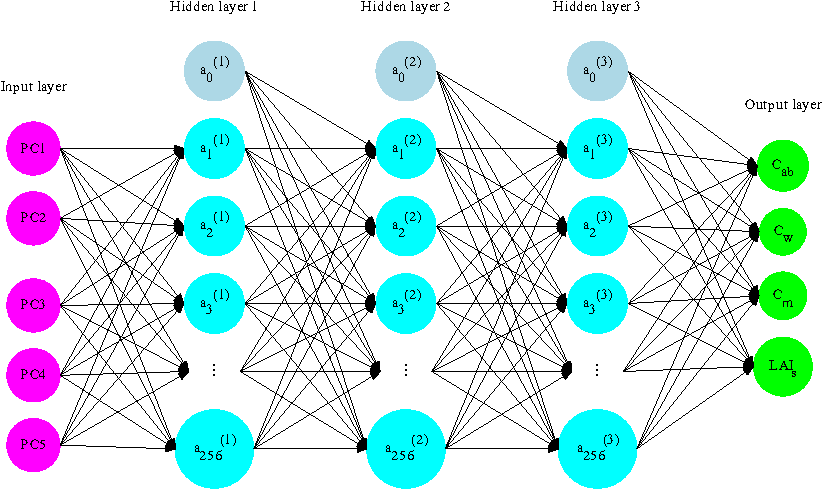
\includegraphics{_main_files/figure-latex/annpca-1.pdf}
\caption{\label{fig:annpca}Architecture of the Neural Network with Principal Components as inputs}
\end{figure}

In the Figure \ref{fig:annpca}, \(a_{n}^{l}\) refers to the \(n\)th unit in the \(l\)th hidden layer. Among all the tested neural network architectures when PCs as an input layer were used, this architecture yielded the best results in terms of the time it took the model to converge, the minimized loss, performance on training, validation and testing sets. However, it is important to note that a different neural network architecture that was not tested in this study could yield better results. Also, slightly simpler architecture could have yielded a similar result if it was trained much longer. But, in this study, simpler architectures (e.g.~NN with 1 or 2 hidden layers) did not perform as well as the chosen architecture (Figure \ref{fig:annpca}) when it was trained for the same number of epochs. It should also be noted that, NN with deeper than 3 hidden layers were not tested in this study.

The Figure \ref{fig:annprisma} shows the chosen NN architecture for the NN model where simulated 231 PRISMA image bands were used as input.

\begin{figure}
\centering
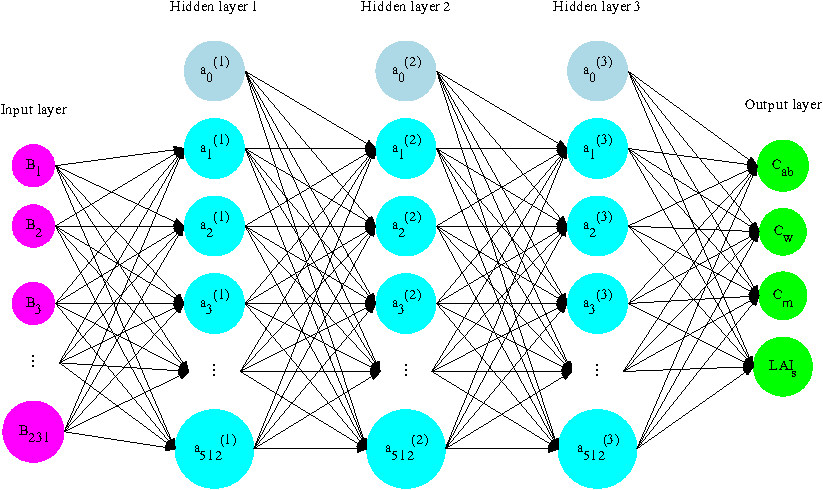
\includegraphics{_main_files/figure-latex/annprisma-1.pdf}
\caption{\label{fig:annprisma}Architecture of the Neural Network with simulated PRISMA image bands as inputs}
\end{figure}

In the Figure \ref{fig:annprisma}, \(B_{n}\) refers to the simulated canopy reflectance for the \(n\)th PRISMA image band and \(a_{n}^{l}\) refers to the \(n\)th unit in the \(l\)th hidden layer. When simulated PRISMA bands were used as an input layer, varying number of hidden layers and number of units had a much more noticeable change. In general, the more complex architectures yielded better results. And, when the NN model with less hidden layers were run for the same or more number of epochs they yielded significantly poorer results. This may potentially indicate that even the more complicated NN architecture could perform better than the chosen architecture.

All of the Neural Network building, testing and training processes were implemented using keras \citep{keras} in tensorflow API \citep{tensorflow}.

\hypertarget{final-prediction-and-map-retrieval}{%
\section{Final prediction and map retrieval}\label{final-prediction-and-map-retrieval}}

Finally, the best performing NN model was used to retrieve \(C_{ab}\), \(C_{w}\), \(C_{m}\) and \(LAI_{s}\) maps for the National Park Hunsrück-Hochwald. Target variables (INFORM parameters) were normalized and standardized using the same Equation \eqref{eq:normy} before training NN models. This means that when we apply the trained NN model to make a prediction on the PRISMA image we get scaled predictions. Therefore, it is necessary to ``un-scale'' the predictions back. To achieve this we can use the Equation \eqref{eq:normy} and scaling (\(\sigma\)) and centering (\(\mu\)) factors of training output variables as follows:

\begin{equation}
Y_{unscaled}\ =\ \left(Y_{predicted_{scaled}}\ \cdot\ \sigma_{Y_{train}\ }\right)\ +\ \mu_{Y_{train}}
\label{eq:unnormy}
\end{equation}

In the Equation \eqref{eq:unnormy} \(Y_{unscaled}\) is the final predicted value, \(Y_{predicted_{scaled}}\) is the scaled version of the prediction, \(\sigma_{Y_{train}}\) is the standard deviation and \(\mu_{Y_{train}}\) is the mean of the corresponding target variable in the training set.

Each pixel in the retrieved maps shows the predicted value of the corresponding INFORM parameter. The final retrieved maps were saved as a 4-band raster file (e.g.~ENVI and Tiff formats) and can be visualized and analysed further.

\hypertarget{results}{%
\chapter{Results}\label{results}}

\hypertarget{local-sensitivity-analysis-1}{%
\section{Local sensitivity analysis}\label{local-sensitivity-analysis-1}}

Figure \ref{fig:fsens} shows the result of sensitivity analysis. Chlorophyll content (\(C_{ab}\)) appears to almost exclusively impact the visible spectra. In general, lower \(C_{ab}\) appears to increase reflectance in the visible spectra. Some effect can also be noticed in the red-edge, but there is not a significant effect of varying \(C_{ab}\) on the simulated spectra within the near-infrared (NIR) and short wave infrared (SWIR) (Figure \ref{fig:fsens}.a). Conversely, equivalent water thickness (\(C_{w}\)) (Figure \ref{fig:fsens}.b) and leaf dry matter content (\(C_{m}\)) (Figure \ref{fig:fsens}.c) both have large effects on simulated spectra within the NIR and SWIR but, no significant effect within the visible spectra. Lower \(C_{w}\) result in higher and lower \(C_{m}\) result in higher simulated canopy reflectance, mainly within the NIR and SWIR. Leaf Area Index (single) (\(LAI_{s}\)) (Figure \ref{fig:fsens}.d), Crown diameter (\(CD\)) (Figure \ref{fig:fsens}.e)) and Stem density (\(SD\)) (Figure \ref{fig:fsens}.f) all have noticeable effect on the simulated canopy reflectance almost all over the spectra. Increased \(LAI_{s}\) result in decreased reflectance. The effects of \(CD\) and \(SD\) on the simulated canopy reflectance is relatively more complex. For example, lower \(CD\) values seem to result in higher reflectance within the visible and SWIR spectra. However, higher values of \(CD\) can also result in higher reflectance mainly within the red-edge and some part of NIR. Increased \(SD\) values appear to result in increased simulated reflectance within the NIR, and decreased reflectance elsewhere.

\newpage

\begin{figure}

{\centering 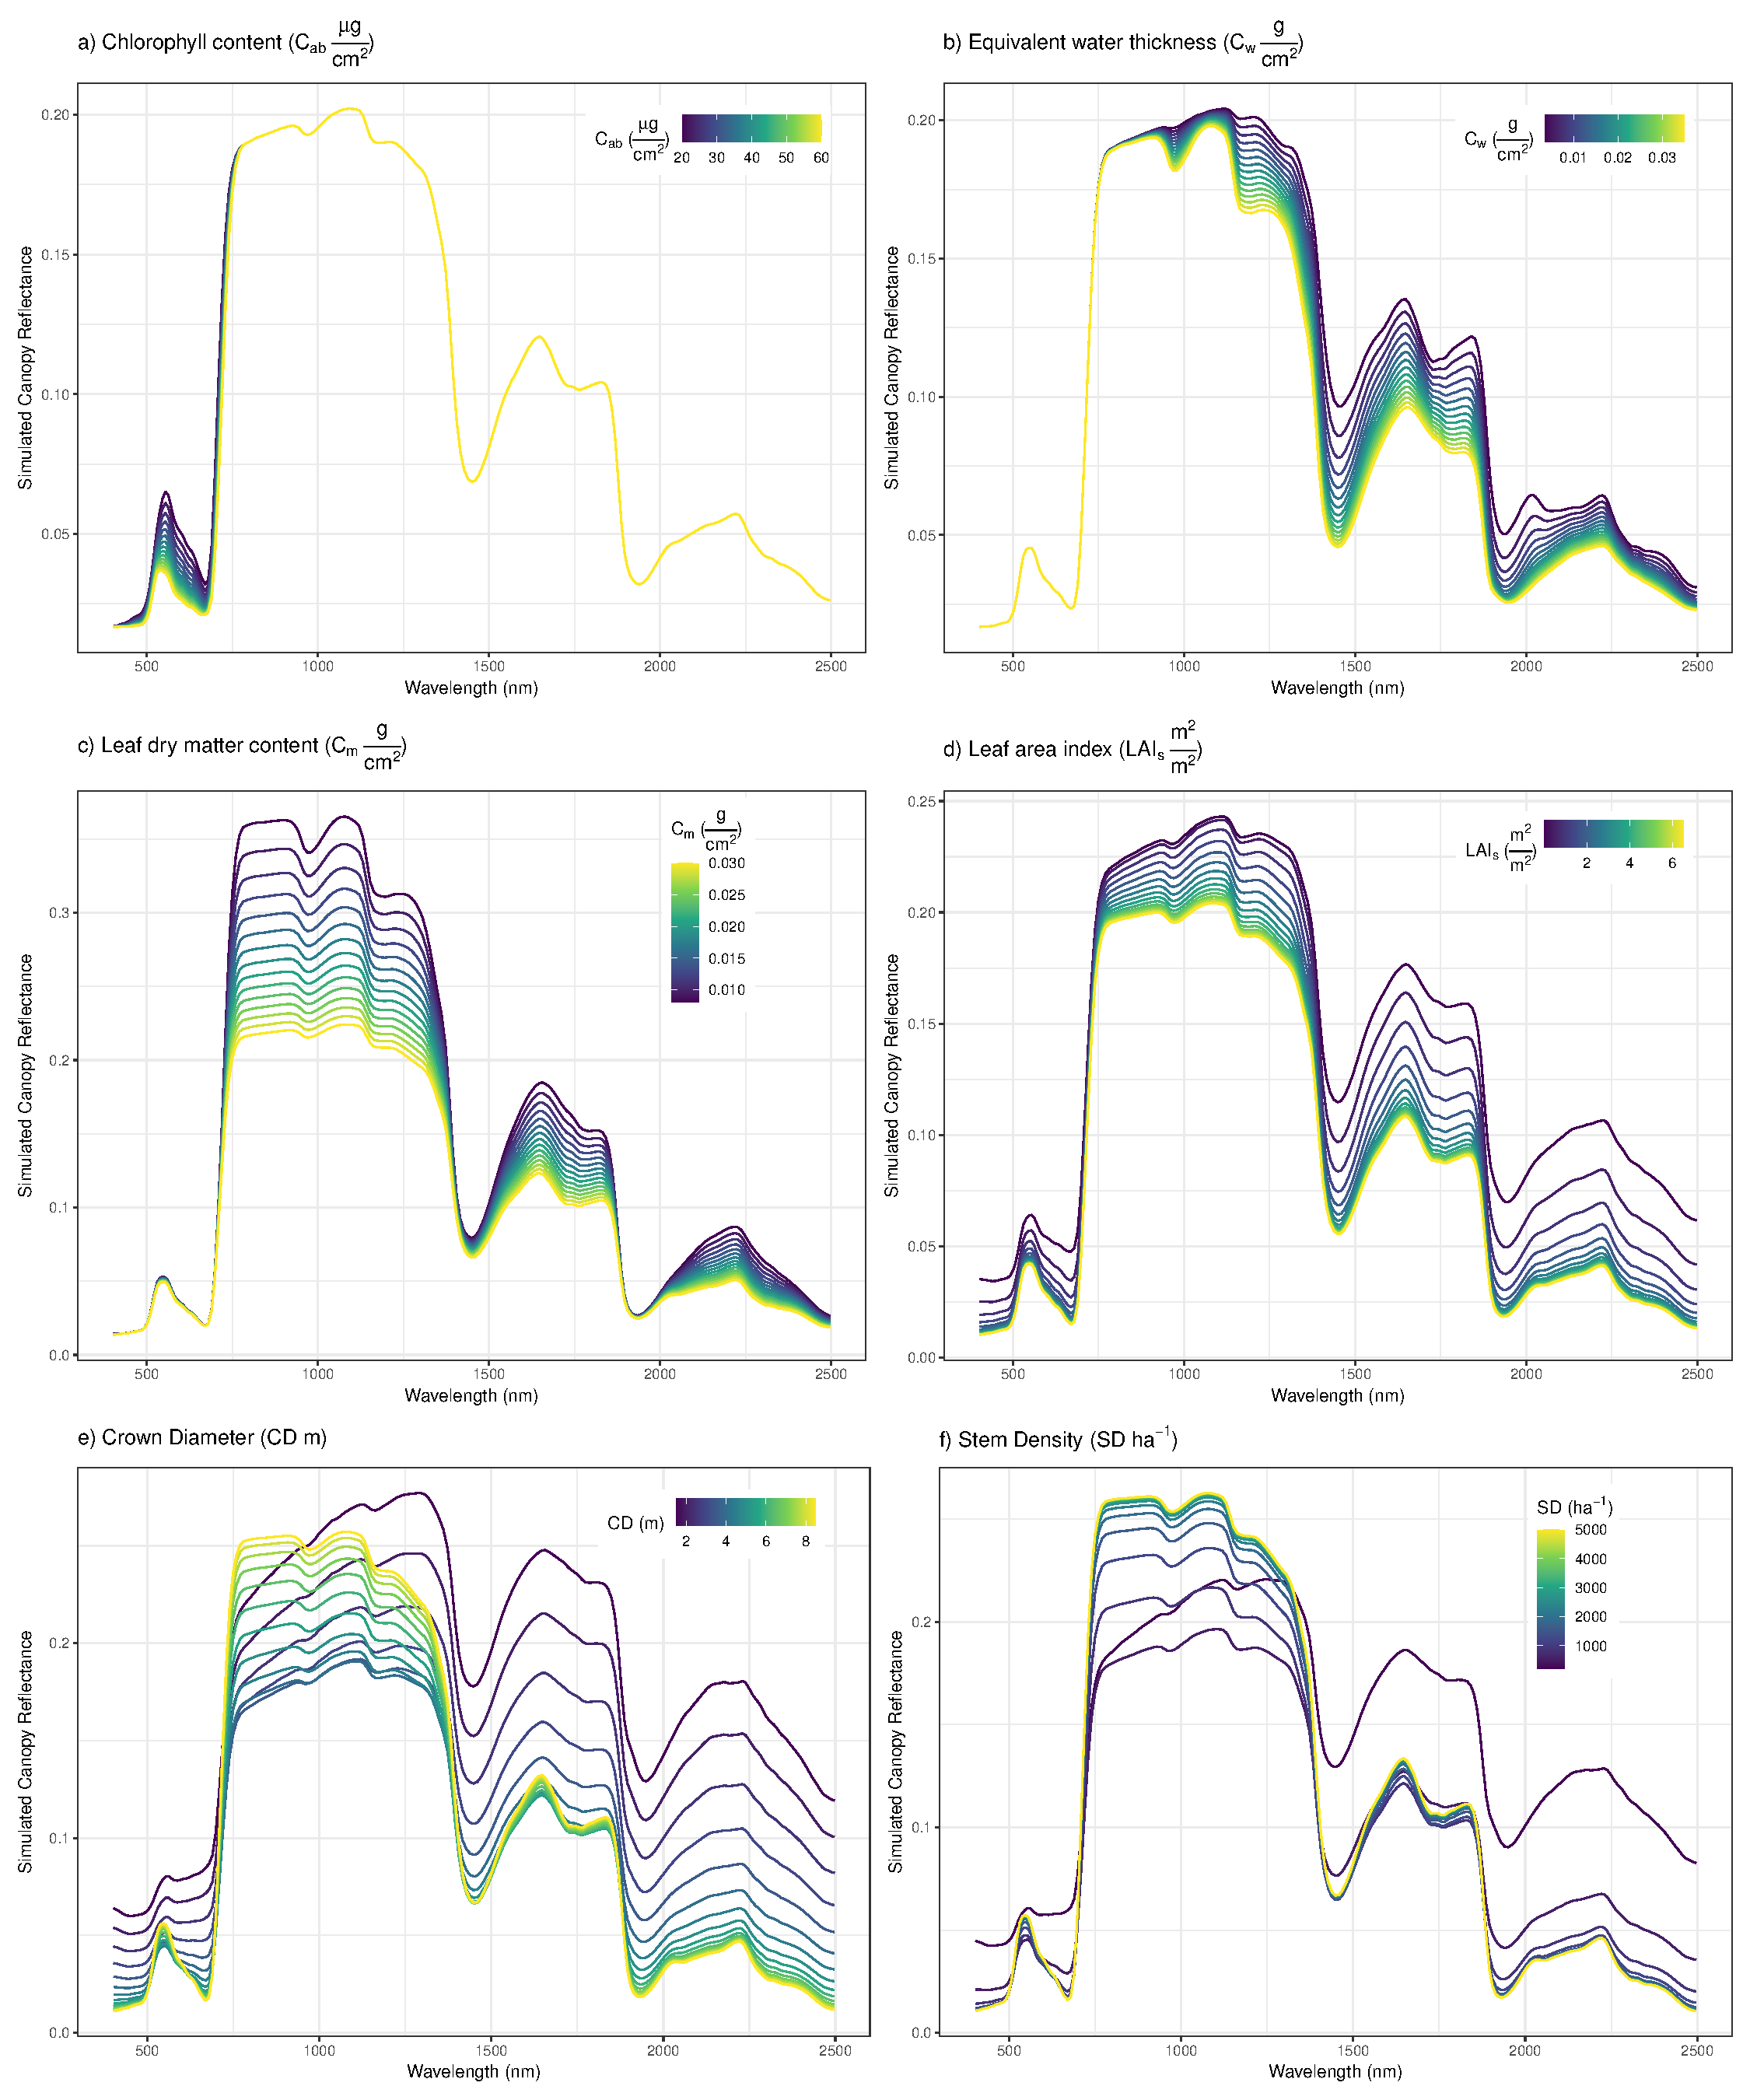
\includegraphics[height=0.8\textheight]{./figures/sensitivity_results} 

}

\caption{Effects of varying the chosen parameters on the simulated spectra}\label{fig:fsens}
\end{figure}

\newpage

\hypertarget{rtm-simulation-inform-1}{%
\section{RTM simulation (INFORM)}\label{rtm-simulation-inform-1}}

Synthetic canopy reflectance data set were produced and stored in a LUT containing all 316,800 simulations. In this research, LUT was defined as a matrix. Each row of this matrix is a different simulated spectra and columns are simulated reflectance of wavelengths with the range of 400nm-2500nm with 1nm spectral resolution and 6 additional columns containing values of the corresponding variables \(C_{ab}\), \(C_{w}\), \(C_{m}\), \(LAI_{s}\), \(CD\) and \(SD\) that were used for each simulation. Hence the dimensions of the LUT matrix is 316,800 rows (number of simulations) by 2107 columns (2101 simulated ``bands'' + 6 INFORM variables):

\begingroup
\tiny

\[
\begin{bmatrix}
400nm_{1} & \dots & 2500nm_{1} & Cab_{1} & Cw_{1} & Cm_{1} & LAIs_{1} & CD_{1} & SD_{1}\\
400nm_{2} & \dots & 2500nm_{2} & Cab_{2} & Cw_{2} & Cm_{2} & LAIs_{2} & CD_{2} & SD_{2}\\
\ \vdots  &\ \vdots &\ \vdots &\ \vdots &\ \vdots &\ \vdots &\ \vdots &\ \vdots &\ \vdots\\
400nm_{316,800} & \dots & 2500nm_{316,800} & Cab_{316,800} & Cw_{316,800} & Cm_{316,800} & LAIs_{316,800} & CD_{316,800} & SD_{316,800}
\end{bmatrix}
\]
\endgroup

In the LUT matrix above, \(400nm_{n}\), \(\dots\), \(2500nm_{n}\) refer to the simulated reflectance for the corresponding wavelength in the simulation number \(n\). \(Cab_{n}\), \(Cw_{n}\), \(Cm_{n}\), \(LAIs_{n}\), \(CD_{n}\) and \(SD_{n}\) are values of the INFORM parameters that were used in the \(n\)th simulation.

\hypertarget{spectral-resampling-1}{%
\section{Spectral resampling}\label{spectral-resampling-1}}

The output of INFORM simulations were resampled to 231 PRISMA bands. The LUT matrix was used for spectral resampling and the resulting matrix has a dimension of 316,800 rows (number of simulations) by 237 columns (231 PRISMA image bands + 6 INFORM variables):

\begingroup
\tiny

\[
\begin{bmatrix}
Band1_{1} & \dots & Band231_{1} & Cab_{1} & Cw_{1} & Cm_{1} & LAIs_{1} & CD_{1} & SD_{1}\\
Band1_{2} & \dots & Band231_{2} & Cab_{2} & Cw_{2} & Cm_{2} & LAIs_{2} & CD_{2} & SD_{2}\\
\ \vdots  &\ \vdots &\ \vdots &\ \vdots &\ \vdots &\ \vdots &\ \vdots &\ \vdots &\ \vdots\\
Band1_{316,800} & \dots & Band231_{316,800} & Cab_{316,800} & Cw_{316,800} & Cm_{316,800} & LAIs_{316,800} & CD_{316,800} & SD_{316,800}
\end{bmatrix}
\]
\endgroup

In this matrix, \(Band1_{n}\), \(\dots\), \(Band231_{n}\) correspond to the simulated reflectance for the corresponding image band in the simulation number \(n\). \(Cab_{n}\), \(Cw_{n}\), \(Cm_{n}\), \(LAIs_{n}\), \(CD_{n}\) and \(SD_{n}\) refer to the values of the INFORM parameters that were used in the \(n\)th simulation.

\hypertarget{statistics-of-simulated-data-and-prisma-image-1}{%
\section{Statistics of simulated data and PRISMA image}\label{statistics-of-simulated-data-and-prisma-image-1}}

The Figure \ref{fig:statplots} shows statistical information (mean and mean \(\pm\) standard deviation) calculated from the LUT and PRISMA image:

\begin{figure}
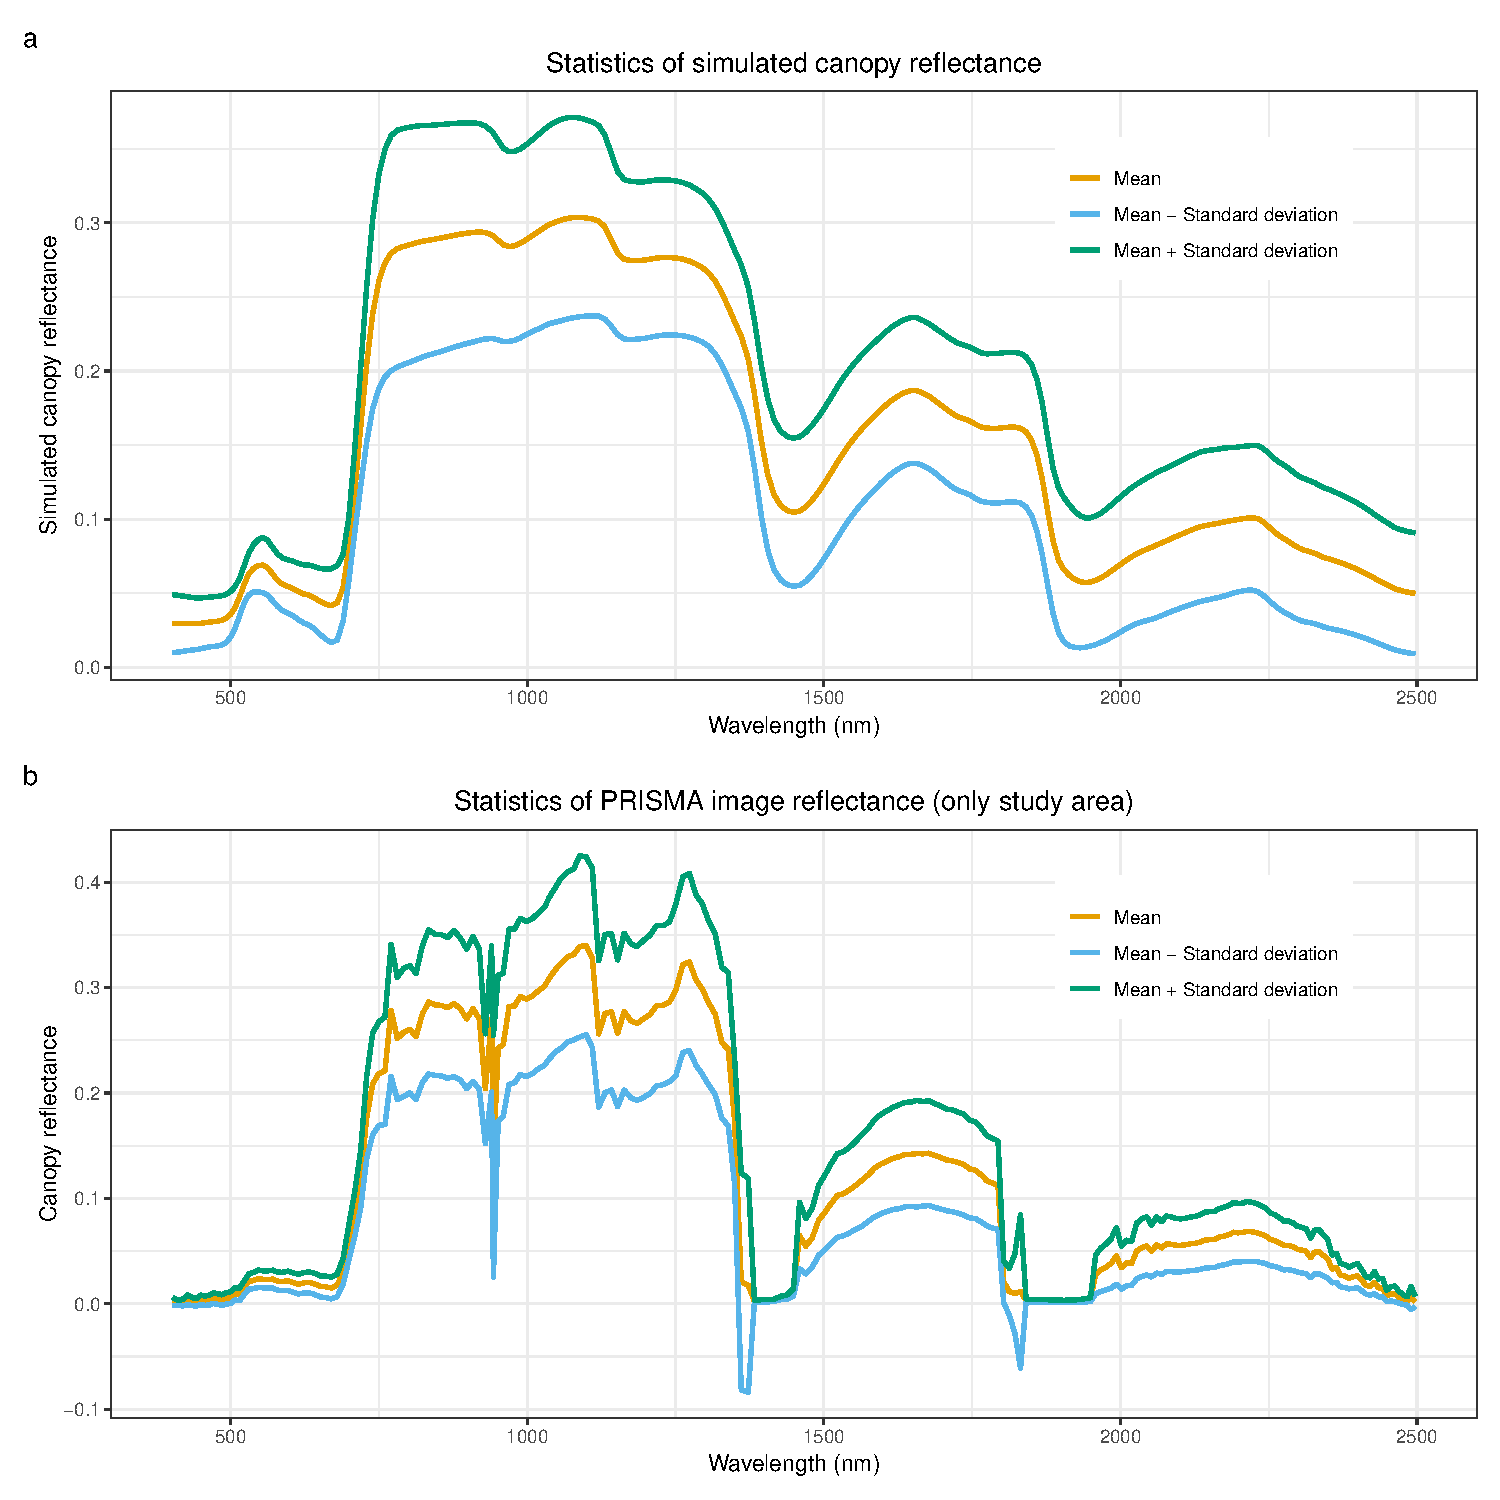
\includegraphics[width=0.9\linewidth]{./figures/stats} \caption{Mean and mean $\pm$ standard deviation in the a) LUT and b) PRISMA image}\label{fig:statplots}
\end{figure}

Mean and standard deviation within the LUT are much smoother compared to mean and standard deviation within the PRISMA image spectra. This is due to the fact that INFORM model does not add noise during the simulation which can commonly exist in remote sensing images. There is a noticeable amount of noise in the PRISMA image spectra. Some of the noise in the image spectra could potentially be due to the fact that the PRISMA image contained cloud and shadow within the study area and although most of the cloud and shadow pixels were masked, the nearby pixels could still be affected.

The Figure \ref{fig:meancomparison} shows the difference between averaged reflectance within the simulated database (LUT) and PRISMA image.

\begin{figure}

{\centering 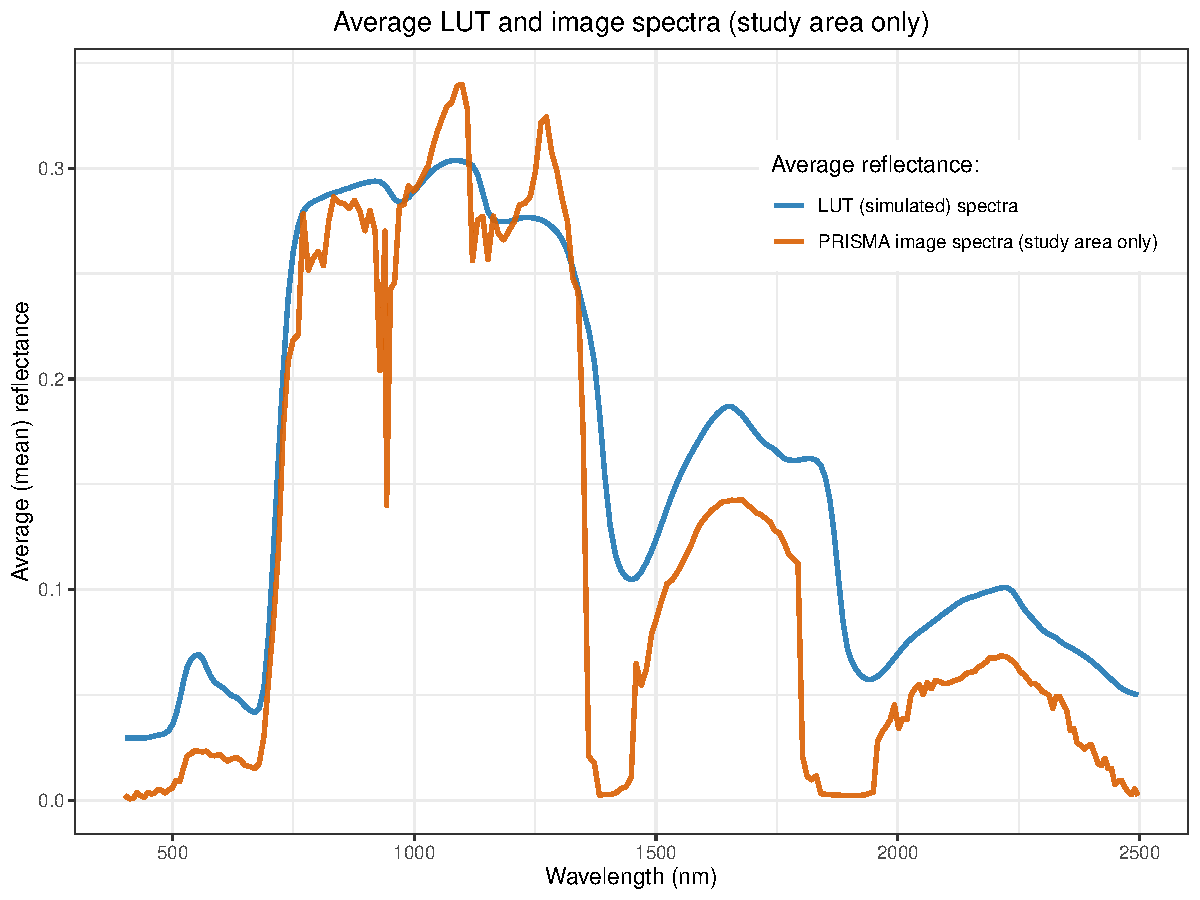
\includegraphics[width=0.8\linewidth]{./figures/meancomparison_lut_vs_prisma} 

}

\caption{Difference between averaged LUT and PRISMA image reflectance}\label{fig:meancomparison}
\end{figure}

The LUT appears to have higher average reflectance within the visible spectra compared to the PRISMA image spectra. Differences within the water absorbtion bands can also be clearly seen. There is relatively good agreement within the NIR spectrum.

\newpage

\hypertarget{gaussian-noise-1}{%
\section{Gaussian noise}\label{gaussian-noise-1}}

The Figure \ref{fig:noise} shows the effect of adding 3\% Gaussian noise to the simulated data.

\begin{figure}
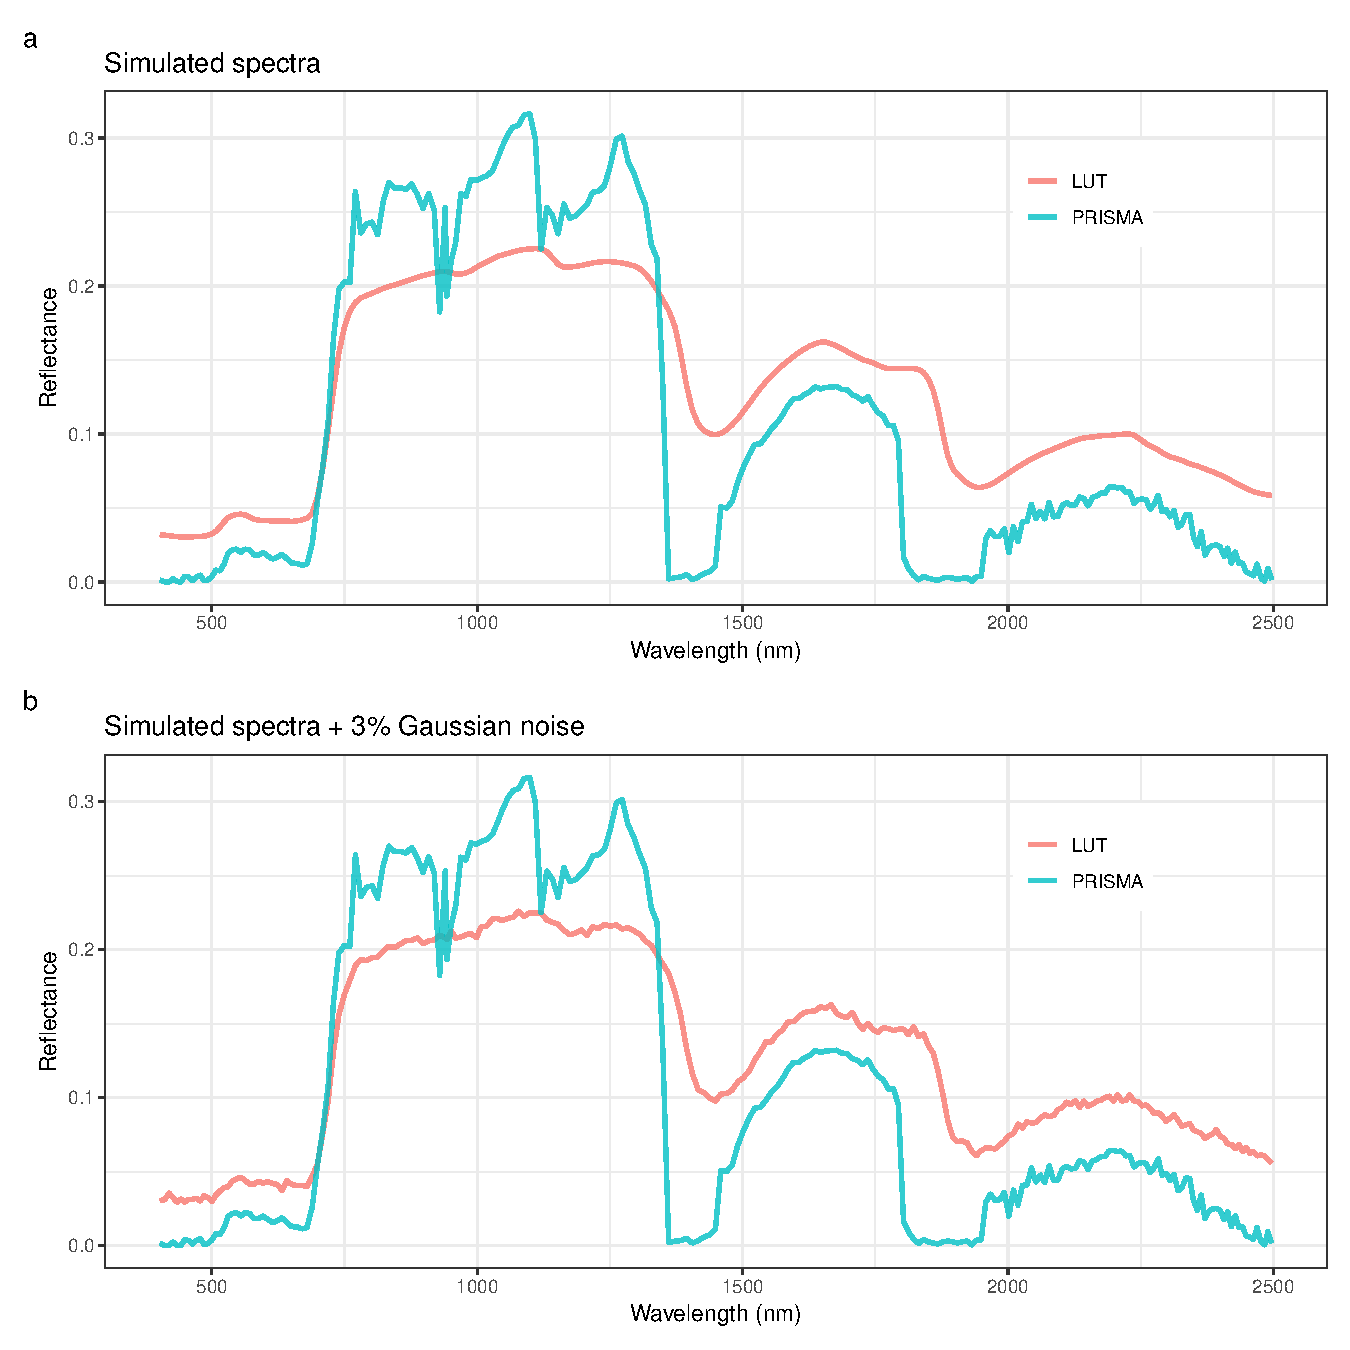
\includegraphics[width=0.9\linewidth]{./figures/noise} \caption{Effect of adding $3\%$ Gaussian noise to the simulated spectra. The randomly chosen pixel from the PRISMA data was plotted to illustrate the noise typically found in the image}\label{fig:noise}
\end{figure}

The Figure \ref{fig:noise}.a shows a simulated spectra that seems perfectly smooth. However, after adding 3\% Gaussian noise, the simulated spectra is not as smooth anymore and contains random noise all over the whole spectra (Figure \ref{fig:noise}.b). This also makes the simulated spectra more similar to the pixel extracted from the PRISMA image.

\hypertarget{principal-component-analysis-pca-1}{%
\section{Principal Component Analysis (PCA)}\label{principal-component-analysis-pca-1}}

The result of PCA show that most of the variation in the simulated data can be explained by much fewer variables (PCs):

\begin{figure}
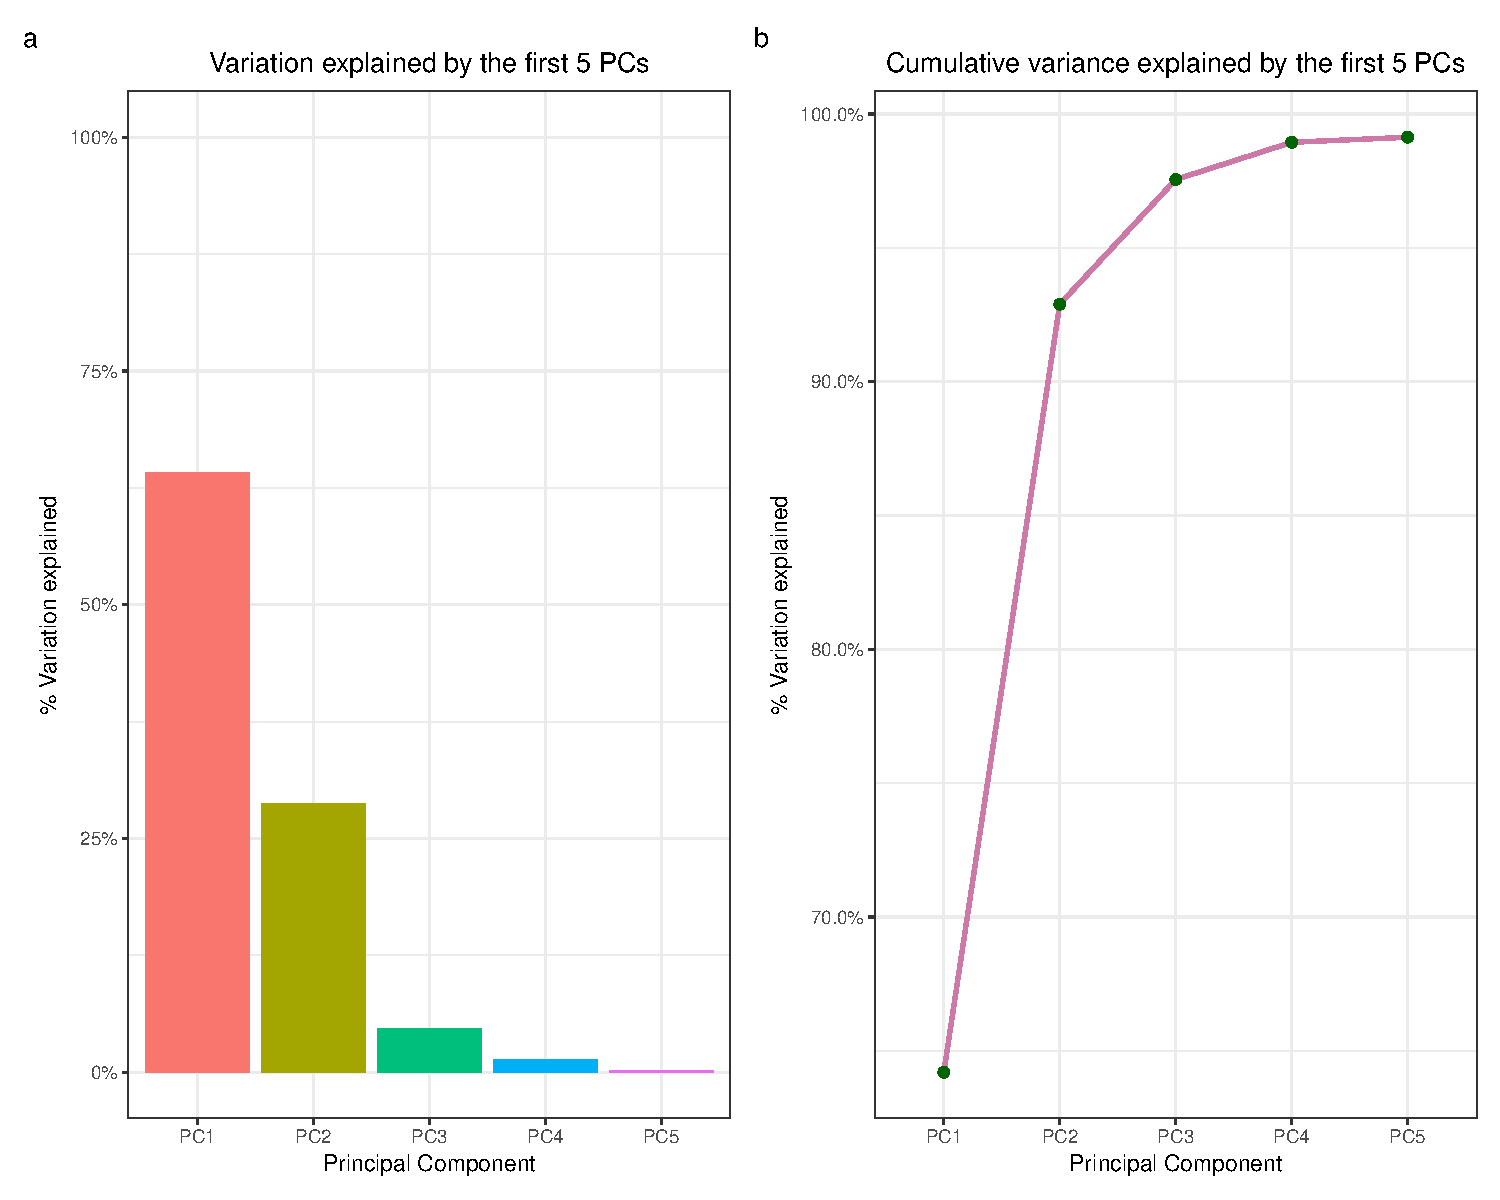
\includegraphics[width=0.9\linewidth]{./figures/pca} \caption{Principal Component Analysis: a) Screeplot, b) Cumulative variance explained by the first 5 PCs}\label{fig:pca}
\end{figure}

The Figure \ref{fig:pca}.a shows the screeplot of the PCA result. The first PC explains the most of the variation and together with the next 4 PCs we can capture more than 99\% of the variation that is present in the original data (Figure \ref{fig:pca}.b). This, once again shows the multicollinearity problem within the hyperspectral data.

\newpage

\hypertarget{artificial-neural-networks-ann-1}{%
\section{Artificial Neural Networks (ANN)}\label{artificial-neural-networks-ann-1}}

\hypertarget{training}{%
\subsection{Training}\label{training}}

The Figure \ref{fig:histannpca} shows the loss, MSE as a function of epochs for the first NN model.

\begin{figure}
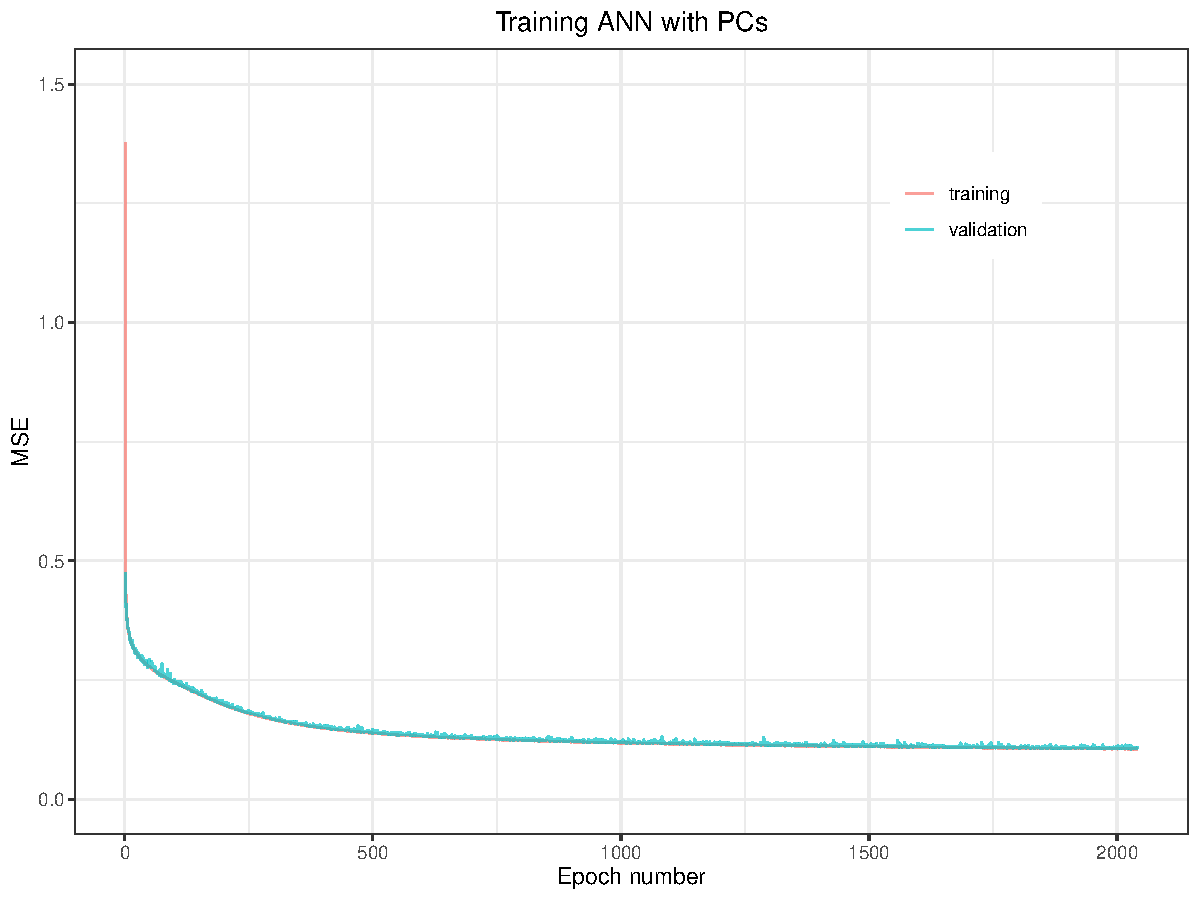
\includegraphics[width=0.9\linewidth]{./figures/hist_annpca} \caption{Training history of ANN with PCs}\label{fig:histannpca}
\end{figure}

It took the NN (when PCs were used as input) more than 2000 epochs to converge to the potential global optima. The loss appears to decrease relatively rapidly during the first 500 epochs. After the epoch number 500 the loss decreases slowly. This may indicate that some of the non-linear relationships between the simulated spectral features and the chosen plant parameters are relatively easy to learn, but the NN needs more training to learn more complicated relationships. The final MSE and MAE this NN achieved when it was evaluated on the testing set was 0.1071568 and 0.1739102 respectively (Table \ref{tab:losstable}). These values are a joint loss of all the target parameters (INFORM parameters).

The Figure \ref{fig:histannrs} shows the training history of the NN where simulated 231 PRISMA bands were used as an input layer.

\begin{figure}
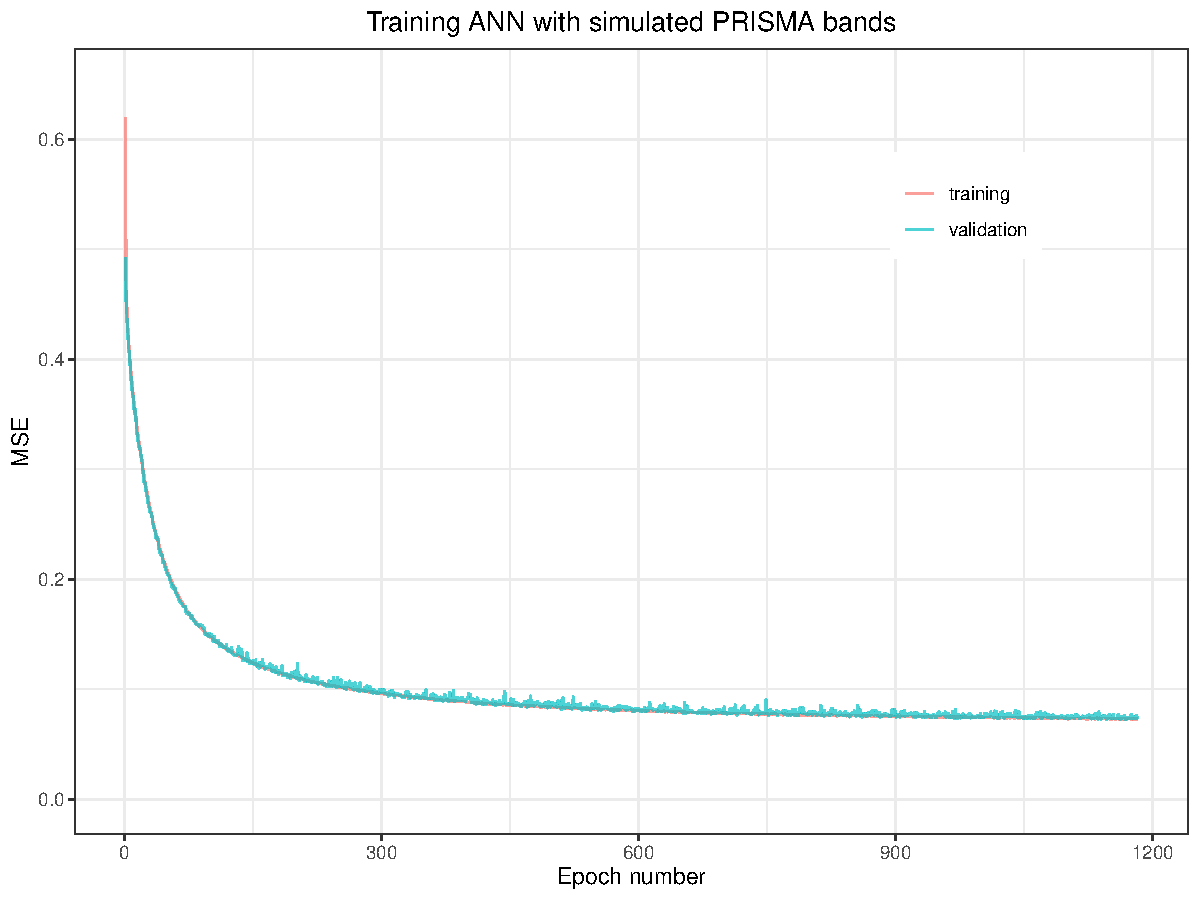
\includegraphics[width=0.9\linewidth]{./figures/hist_annrs} \caption{Training history of ANN with simulated PRISMA bands}\label{fig:histannrs}
\end{figure}

In this model, less than 1200 epochs of training was enough for the NN to converge. Also, the training, validation and most importantly, testing losses were lower (compared to the first NN) when the simulated PRISMA bands were used as predictors (Table \ref{tab:losstable}).

The lines that show training and validation loss over epochs (Figures \ref{fig:histannpca} and \ref{fig:histannrs}) are close to each other and show more or less similar pattern of decrease. This is a sign that there is no a serious overfitting problem during the training. Before adding regularization term to the cost function, however, there was sign of overfitting during the training.

\newpage

The Table \ref{tab:losstable} summarizes the final results of the ANNs.

\begin{table}[H]

\caption{\label{tab:losstable}Final results of the trained NNs}
\centering
\begin{tabular}[t]{llll}
\toprule
Dataset & Metric & NN with PCs & NN with sim. bands\\
\midrule
Train & MSE & 0.1049012 & 0.07522584\\
Train & MAE & 0.1710693 & 0.13174930\\
Validation & MSE & 0.1068904 & 0.07499193\\
Validation & MAE & 0.1740899 & 0.13256425\\
Test & MSE & 0.1071568 & 0.07670474\\
\addlinespace
Test & MAE & 0.1739102 & 0.13459726\\
\bottomrule
\end{tabular}
\end{table}

This result indicates that, when designing the NN architecture properly and giving reasonable amount of hidden layers and units, the NN model can deal with multicollinearity very efficiently.

\hypertarget{evaluation-of-the-nn-models-on-the-testing-set}{%
\subsection{Evaluation of the NN models on the testing set}\label{evaluation-of-the-nn-models-on-the-testing-set}}

The Figure \ref{fig:predstest} shows the scatterplots of the predicted parameters versus modelled parameters for the PCA based NN (first column or the plots on the left side) and NN with simulated PRISMA bands (the second column or the plots on the right). For easier visualization of the scatter plots only 1500 data points were randomly sampled from the testing data set (full testing data could be too large to visualize). Also, there was an overplotting problem in the original scatter plots due to many similar points laying on top of each other. Therefore, the ``jitter'' technique was used, which adds a very small random noise to each point (location wise) that makes visualization easier \citep{wickham2016r, ggplot2}. The blue diagonal line shows the 1:1 line that has an intercept 0 and slope 1.

\newpage

\begin{figure}
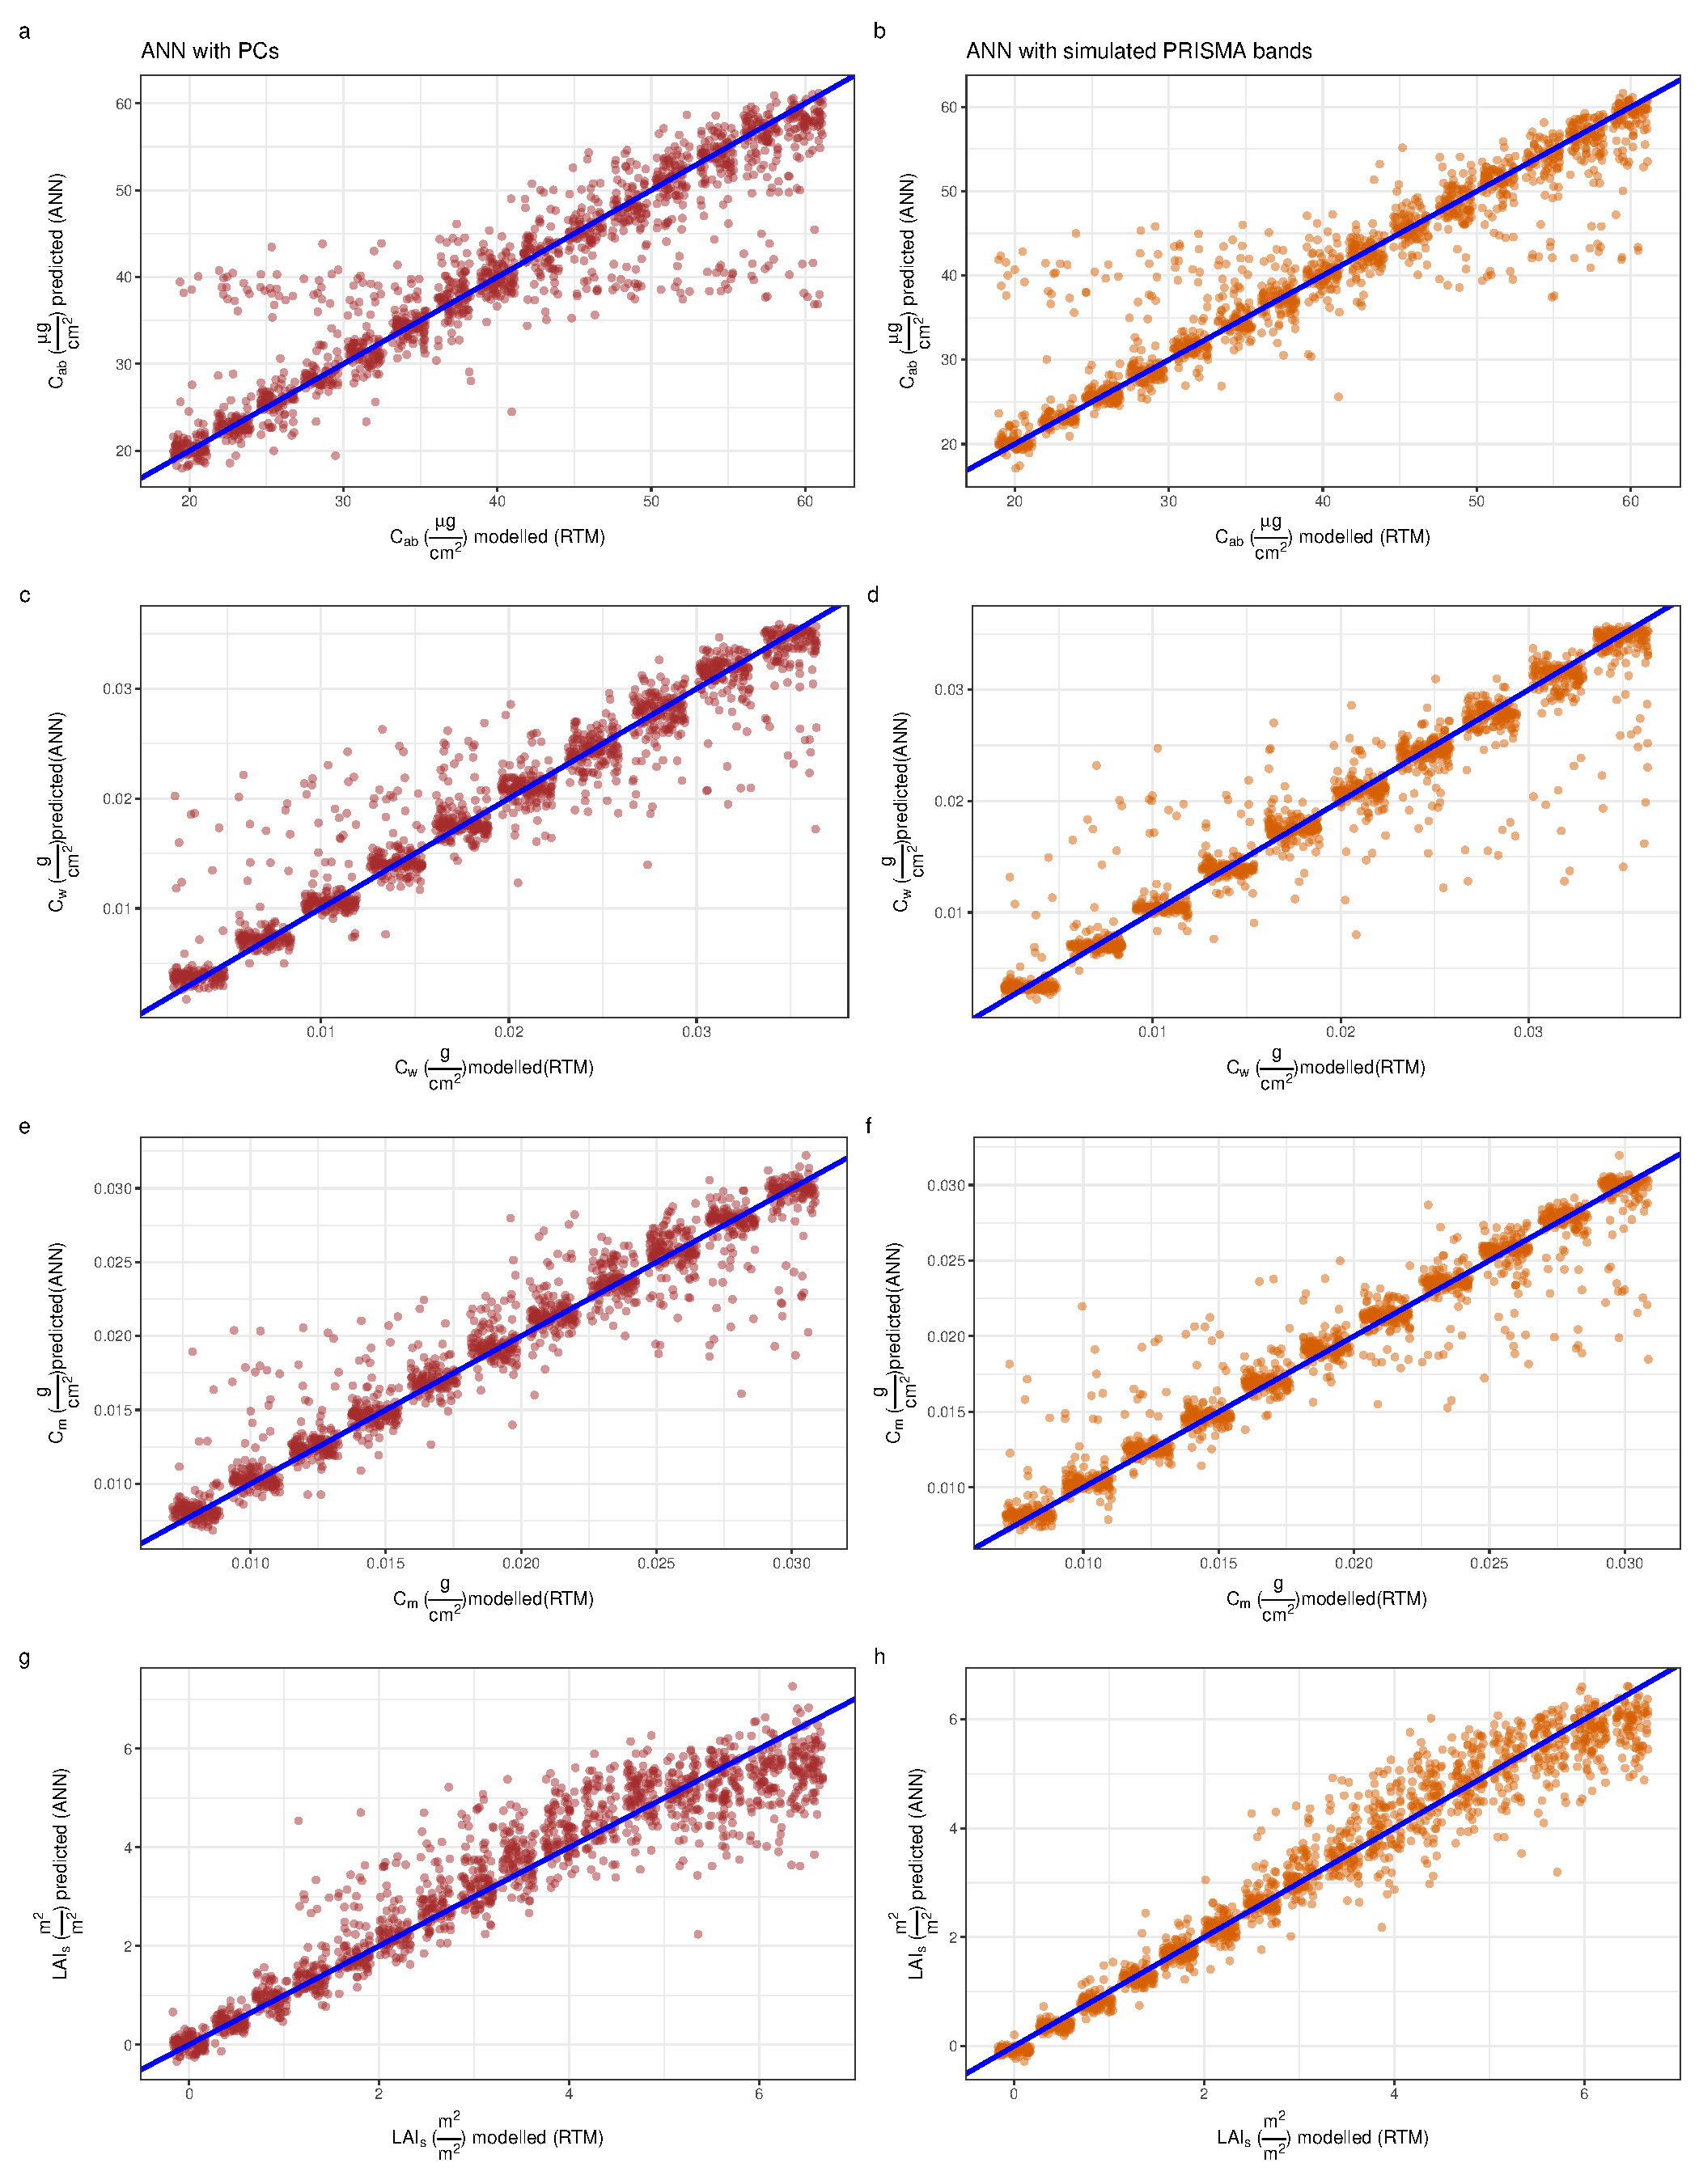
\includegraphics[width=1\linewidth]{./figures/preds_test} \caption{Predicted versus modelled RTM parameters for the PCA based NN (1st column) and NN with simulated PRISMA bands (2nd column)}\label{fig:predstest}
\end{figure}

In general, both of the NN models appears to perform well on the testing set that it was not trained on. The effect of adding random Gaussian noise can clearly be seen. The points that are relatively far from the diagonal line are results of adding 3\% Gaussian noise. This was not the case on the NN model that was trained with simulated data that did not receive any amount of noise. The parameter \(C_{ab}\) appears to be impacted by the noise more significantly compared to other paramters. This is potentially due to the fact that \(C_{ab}\) has a very specialized impact on the simulated reflectance, almost exclusively on the visible spectra (Figure \ref{fig:fsens}.a). Unlike \(C_{ab}\), the other parameters had impact on more bands (Figure \ref{fig:fsens}) and this might have helped the NN learn the relationship more easily for these parameters despite the existence of noise.

Although overall pattern seems very similar, accuracy of the NN model that was trained with simulated image bands is slightly better for all the parameters. Superiority of this NN model is more noticeable for the parameter \(LAI_{s}\) (Figure \ref{fig:predstest}.h). The Table \ref{tab:modelacc} shows the differences between the results of the two models on the testing set parameters.

\begin{table}[H]

\caption{\label{tab:modelacc}Differences between the performances of the trained 2 NN models on the testing set parameters}
\centering
\begin{tabular}[t]{lllll}
\toprule
Parameter & $R^{2}$ (PCs)\textsuperscript{*} & RMSE (PCs)\textsuperscript{*} & $R^{2}$ (Bands)\textsuperscript{\dag} & RMSE (Bands)\textsuperscript{\dag}\\
\midrule
$C_{ab}$ & 0.8733358 & 4.37369 ($\frac{\mu g}{cm^2}$) & 0.8911385 & 4.064 ($\frac{\mu g}{cm^2}$)\\
$C_{cw}$ & 0.9246098 & 0.002765111 ($\frac{g}{cm^2}$) & 0.9396872 & 0.00252202 ($\frac{g}{cm^2}$)\\
$C_{cm}$ & 0.9341707 & 0.001798028 ($\frac{g}{cm^2}$) & 0.9428488 & 0.001702862 ($\frac{g}{cm^2}$)\\
$LAI_{s}$ & 0.896475 & 0.641572 ($\frac{m^2}{m^2}$) & 0.9513208 & 0.443341 ($\frac{m^2}{m^2}$)\\
\bottomrule
\multicolumn{5}{l}{\rule{0pt}{1em}\textsuperscript{*} PCs - refers to the result of NN with Principal Components}\\
\multicolumn{5}{l}{\rule{0pt}{1em}\textsuperscript{\dag} Bands - refers the result of NN with simulated PRISMA bands}\\
\end{tabular}
\end{table}

The NN trained with simulated 231 PRISMA bands predicts INFORM parameters \(C_{ab}\), \(C_{w}\) and \(C_{m}\) with slightly better \(R^{2}\) and \(RMSE\). This NN model predicts \(LAI_{s}\) with much better accuracy. This could potentially be due to the fact that \(LAI_{s}\) has an important effect within the full spectra (see sensitivity subplot Figure \ref{fig:fsens}.d) and the 5 PCs do not properly represent the full relationship between the plant parameter \(LAI_{s}\) and spectra.

\hypertarget{final-prediction-and-map-retrieval-1}{%
\section{Final prediction and map retrieval}\label{final-prediction-and-map-retrieval-1}}

The NN that was trained with 231 simulated PRISMA bands was used for map retrieval as the final optimal model. Four different maps for the parameters \(C_{ab}\), \(C_{w}\), \(C_{m}\) and \(LAI_{s}\) were produced as raster images. Each pixel in the retrieved maps is the predicted value of the corresponding INFORM parameter.

\hypertarget{retrieval-of-c_ab-map}{%
\subsection{\texorpdfstring{Retrieval of \(C_{ab}\) map}{Retrieval of C\_\{ab\} map}}\label{retrieval-of-c_ab-map}}

The Figure \ref{fig:mapcab} shows the predicted map of the parameter \(C_{ab}\).

\begin{figure}
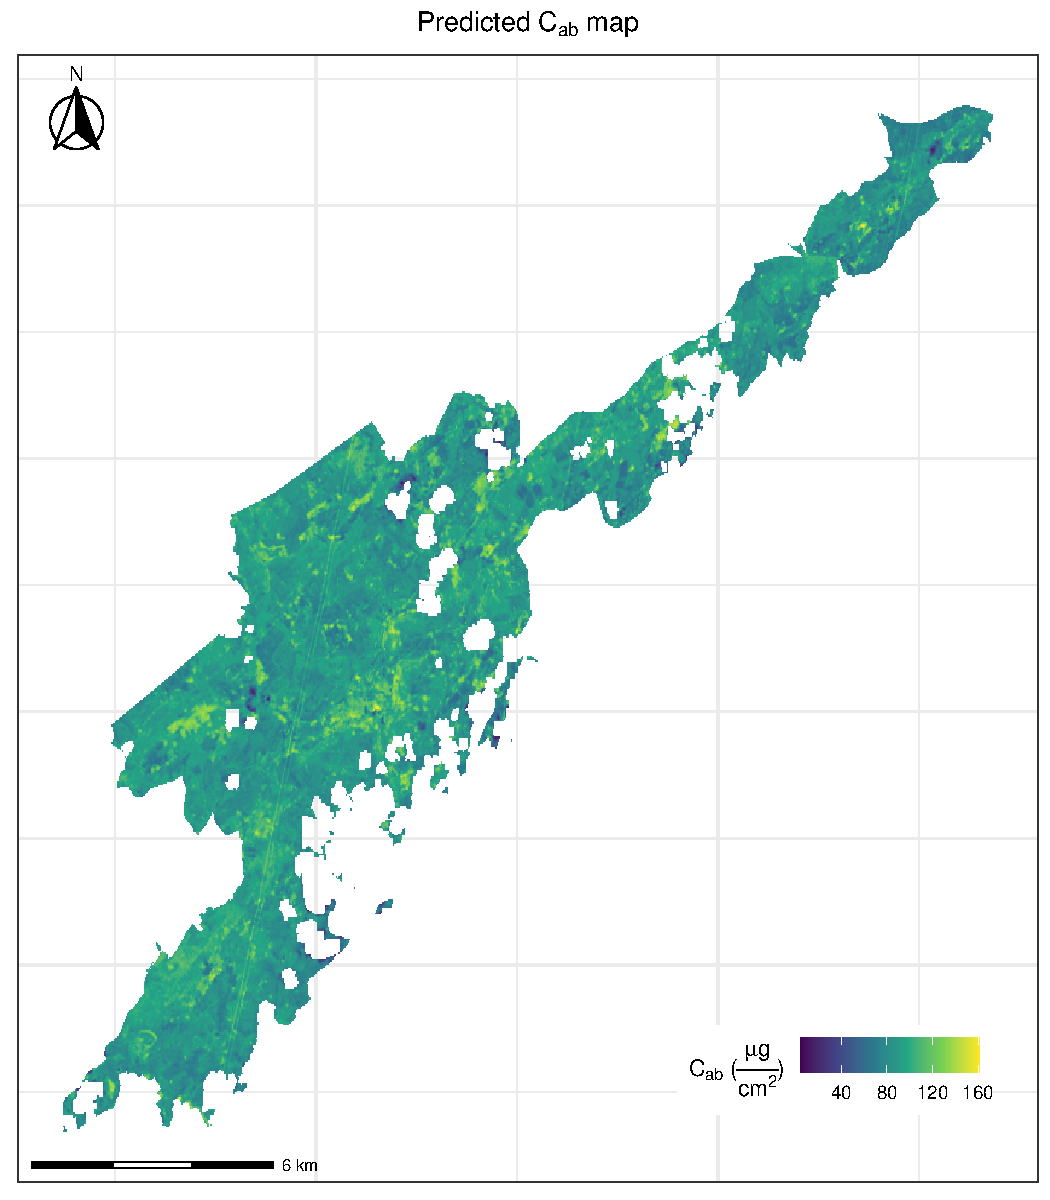
\includegraphics[width=0.9\linewidth]{./figures/cab_map} \caption{Predicted map of the parameter $C_{ab}$}\label{fig:mapcab}
\end{figure}

Although there are some pixels showing values that are similar to the range that was used during the RTM simulation, some pixels show higher \(C_{ab}\) values than the values that were used for simulation. This is further supported by the Figure \ref{fig:histcab}.

\begin{figure}
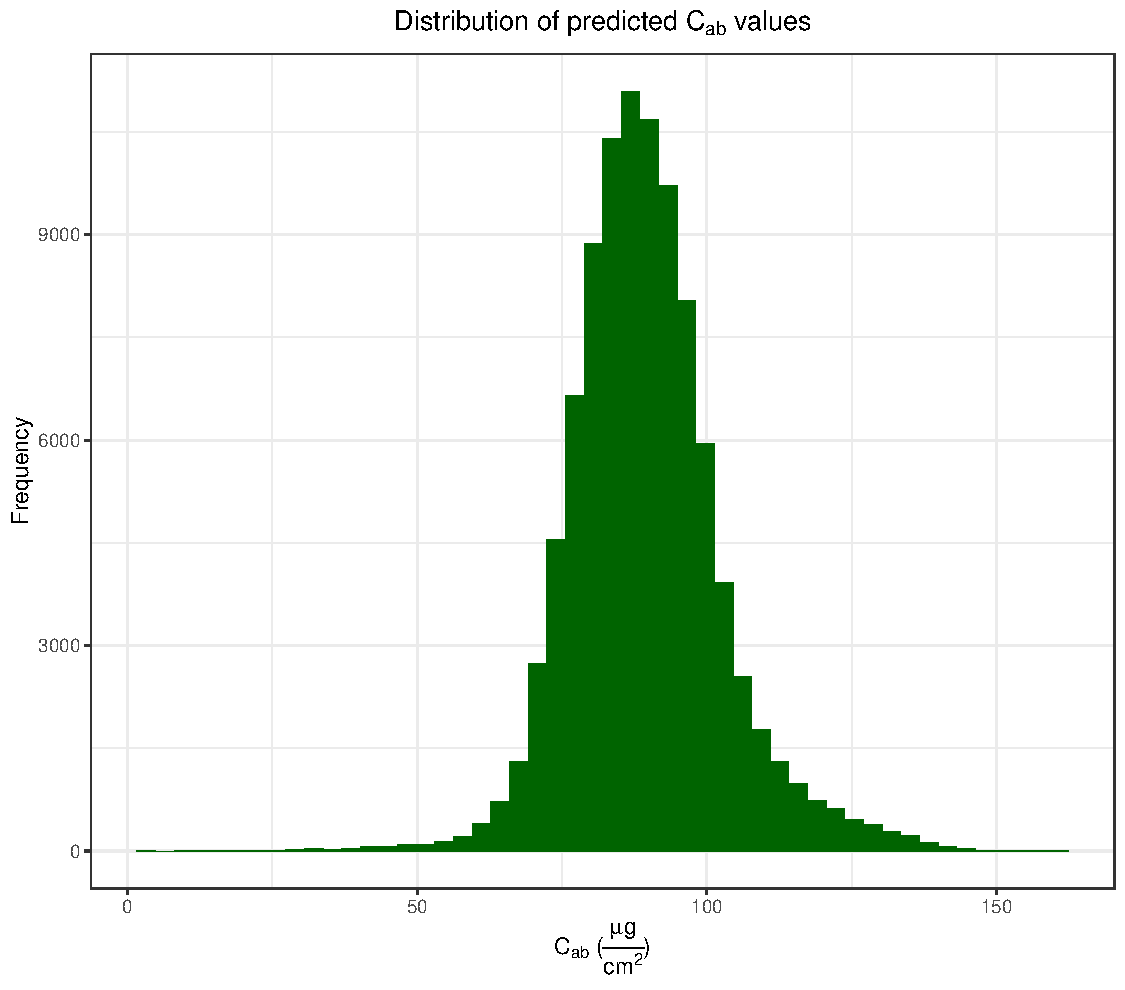
\includegraphics[width=0.8\linewidth]{./figures/cab_hist} \caption{Distribution of the predicted values for the parameter $C_{ab}$}\label{fig:histcab}
\end{figure}

The reason why the trained NN predicts higher values for the PRISMA image compared to the value range that was used in the simulation can be explained by the fact that the parameter \(C_{ab}\) only have a significant impact on the visible spectra (see Figure \ref{fig:fsens}.a) and average reflectance in the visible spectra of the PRISMA image is lower compared to the average reflectance of the visible spectra in the LUT (simulated database) (see Figure \ref{fig:meancomparison}). Specifically, the sensitivity analysis showed that the higher the \(C_{ab}\) value, the lower the reflectance in the visible spectra will be (Figure \ref{fig:fsens}.a). This means that it is expected to get higher predicted \(C_{ab}\) values for the PRISMA image.

\hypertarget{retrieval-of-c_w-map}{%
\subsection{\texorpdfstring{Retrieval of \(C_{w}\) map}{Retrieval of C\_\{w\} map}}\label{retrieval-of-c_w-map}}

The Figure \ref{fig:mapcw} shows the predicted map of the parameter \(C_{w}\).

\begin{figure}
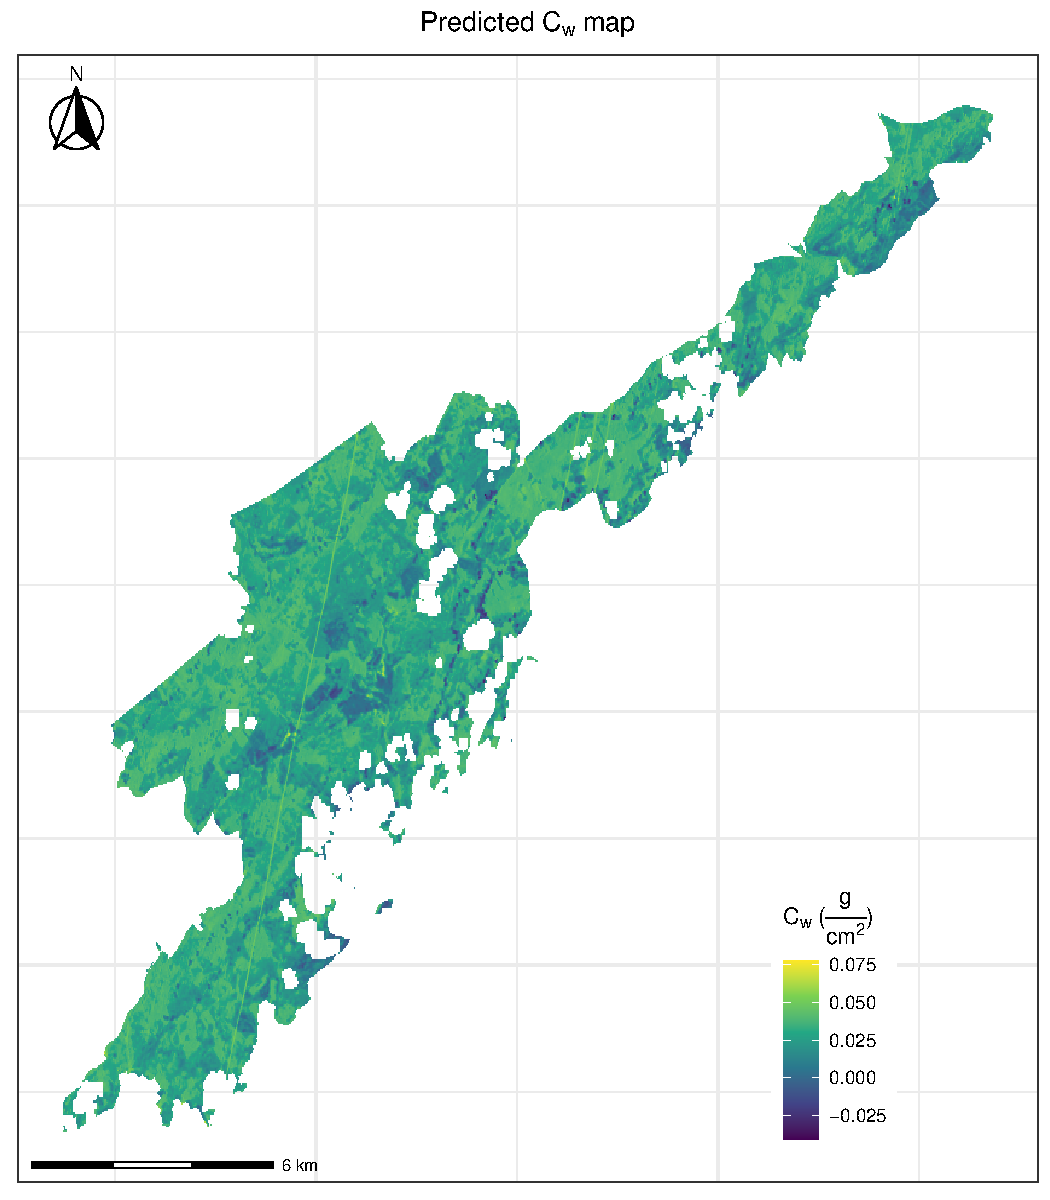
\includegraphics[width=0.9\linewidth]{./figures/cw_map} \caption{Predicted map of the parameter $C_{w}$}\label{fig:mapcw}
\end{figure}

Majority of the pixels show predicted values that are within the same range of the values used during the simulation. The parameter \(C_{w}\) has a large effect on the NIR spectrum (Figure \ref{fig:fsens}.b) and the average reflectance in the NIR region within both LUT and PRISMA image are relatively close to each other (Figure \ref{fig:meancomparison}). This could explain why the range of the predicted \(C_{w}\) values is similar to the \(C_{w}\) range within the LUT. However, there is also a large impact of \(C_{w}\) on the SWIR and this region of the average simulated spectra is higher than the average reflectance of SWIR in the PRISMA image spectra.

The Figure \ref{fig:histcw} shows the distribution of the predicted \(C_{w}\) values in more detail.

\begin{figure}
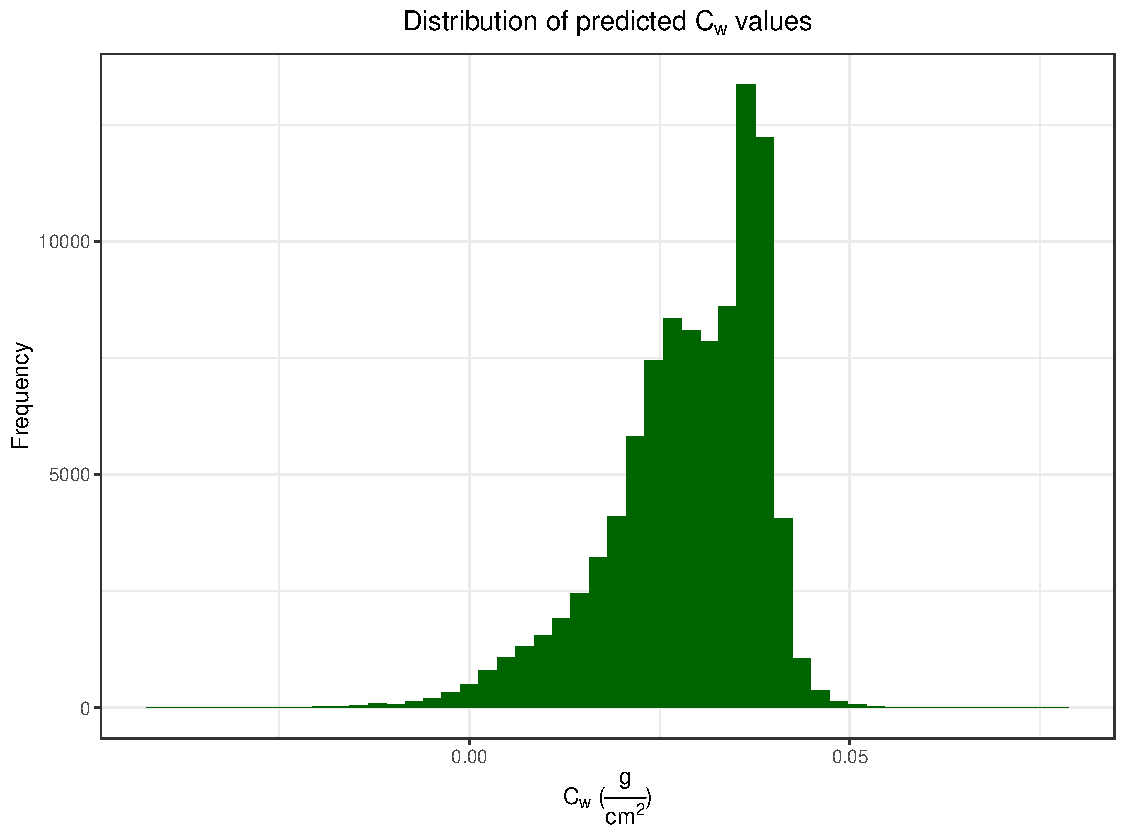
\includegraphics[width=0.8\linewidth]{./figures/cw_hist} \caption{Distribution of the predicted values for the parameter $C_{w}$}\label{fig:histcw}
\end{figure}

\newpage

\hypertarget{retrieval-of-c_m-map}{%
\subsection{\texorpdfstring{Retrieval of \(C_{m}\) map}{Retrieval of C\_\{m\} map}}\label{retrieval-of-c_m-map}}

The Figure \ref{fig:mapcm} shows the predicted map of the parameter \(C_{m}\).

\begin{figure}
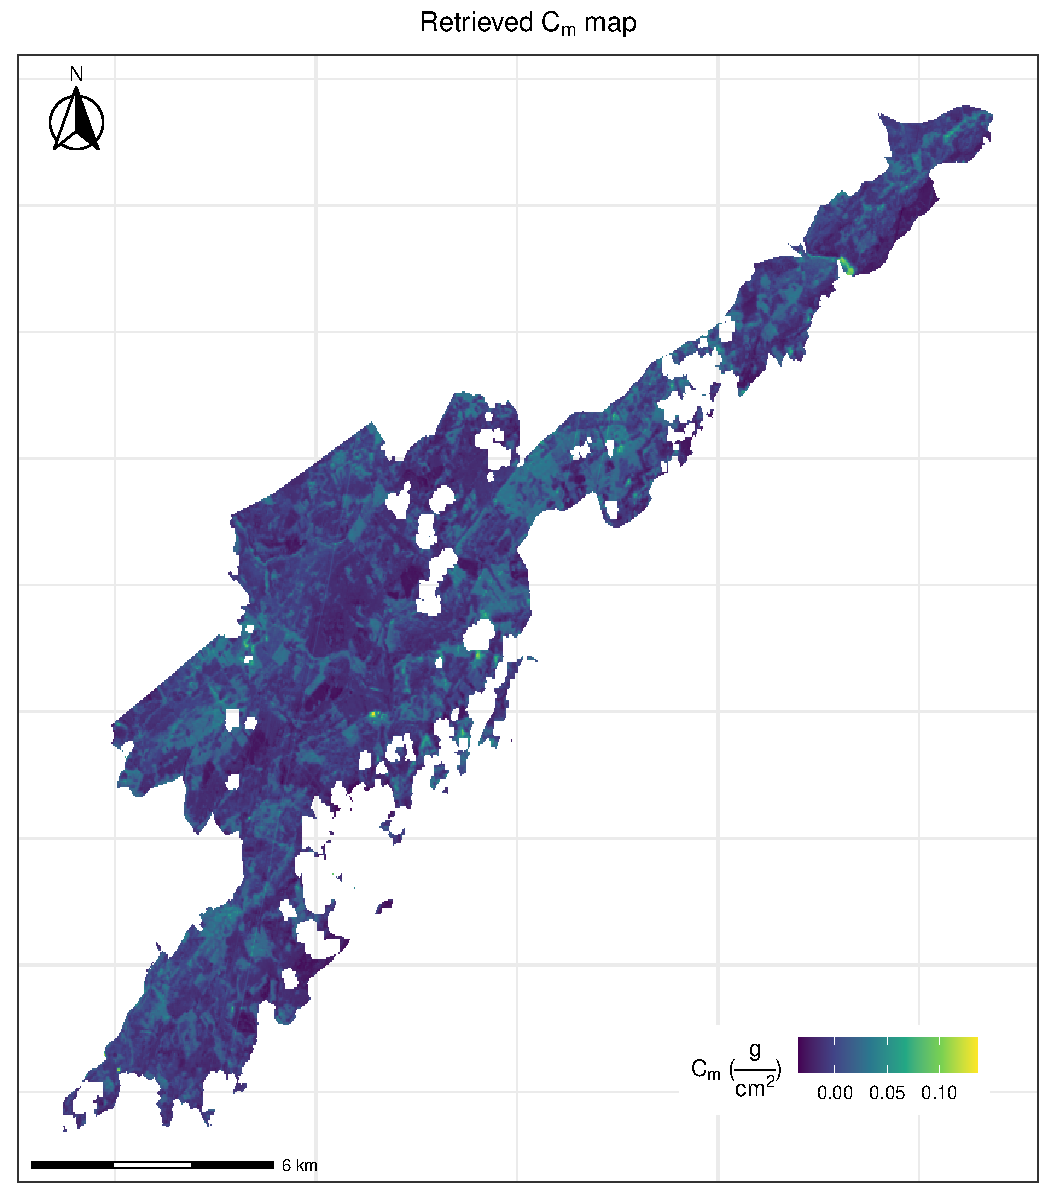
\includegraphics[width=0.9\linewidth]{./figures/cm_map} \caption{Predicted map of the parameter $C_{m}$}\label{fig:mapcm}
\end{figure}

The predicted \(C_{m}\) map shows that some of the pixels in the predicted map is smaller than 0. The sensitivity analysis showed that increased \(C_{m}\) values decreases the reflectance over NIR and SWIR (Figure \ref{fig:fsens}.c). In average, the PRISMA image pixels have lower reflectance within the SWIR region of the spectra and this is the reason why the trained NN predicts low values \(C_{m}\) for some of the pixels.

\hypertarget{retrieval-of-lai_s-map}{%
\subsection{\texorpdfstring{Retrieval of \(LAI_{s}\) map}{Retrieval of LAI\_\{s\} map}}\label{retrieval-of-lai_s-map}}

The Figure \ref{fig:maplai} shows the predicted map of the parameter \(LAI_{s}\).

\begin{figure}
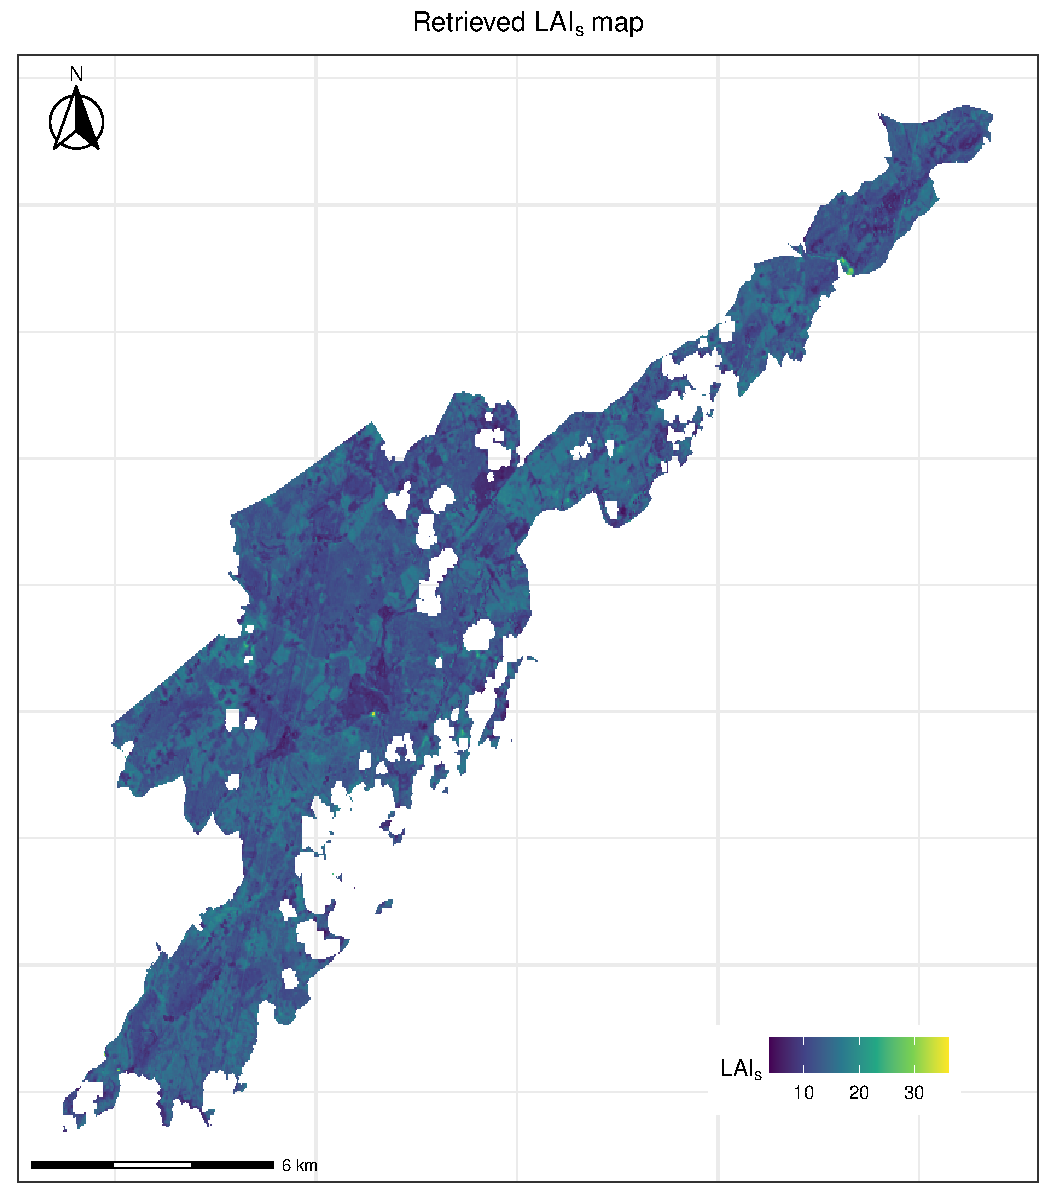
\includegraphics[width=0.9\linewidth]{./figures/lais_map} \caption{Predicted map of the parameter $LAI_{s}$}\label{fig:maplai}
\end{figure}

We can see that most of the pixels in the predicted \(LAI_{s}\) map show the value range of 10-15.

\hypertarget{discussion}{%
\chapter{Discussion}\label{discussion}}

In this study, first the RTM model INFORM was used to simulate forest canopy reflectance and then, the simulated data was used to train ANN model in order for it to predict the studied plant traits of the hyperspectral remote sensing imagery. This section discusses the results and further improvements.

\hypertarget{artificial-neural-networks-for-predicting-plant-traits}{%
\section{Artificial Neural Networks for predicting plant traits}\label{artificial-neural-networks-for-predicting-plant-traits}}

This study showed that, given enough hidden layers and neurons, using artificial neural networks can efficiently deal with high multi-collinearity that exist within hyperspectral remote sensing data to predict plant biophysical and biochemical parameters. For all the INFORM parameters the NN that was trained with simulated 231 PRISMA bands had better results compared to the NN that was trained with 5PCs. Training NN with full image bands to predict plant biophysical and biochemical parameters that have effect within the whole spectra (e.g.~LAI) could specifically be beneficial. However, it should also be noted that, depending on the availability of the computational resources and time, using a dimensionality reduction technique such as PCA may be preferred. This is because training NN with hundreds of predictors (e.g.~hyperspectral image bands) usually needs more time to run compared to a PCA based NN that is trained with only several predictors (principal components). However, in this study, for the NN that was trained with hyperspectral image bands it took less than 1200 epochs to converge, while the PCA based NN needed to run more than 2000 epochs. This could potentially indicate that for the NN it may be easier to learn the relationships between the plant traits and simulated spectra when all the bands are available. The design of the NN had a significant effect on the results and predictions. Neural networks with simpler architecture led to poor performance, while relatively deeper NN architecture had good prediction accuracies for the plant parameters.

\hypertarget{further-improvements}{%
\section{Further improvements}\label{further-improvements}}

This model, that was built with the help of RTM and machine learning, can be used to predict the plant traits \(C_{ab}\), \(C_{w}\), \(C_{m}\) and \(LAI_{s}\) in the hyperspectral remote sensing data PRISMA. These plant traits could be very beneficial to study forest disturbances especially for Spruce trees.

Potential follow up study could be to use this model in order to retrieve forest biochemical and biophysical maps from the hyperspectral data PRISMA for multiple dates. Then, scientific techniques like change detection could be applied to assess the change of these variables between multiple years.

It is also important to mention that this model could still be improved further. For example, using destructive and non-destructive in-situ data for RTM simulations could potentially lead to better results. In this study, these types of data were not available and the referenced literature was used to choose the range of values for RTM simulation. This data could also help assess the performance of the models (RTM and ANN) in more detail.

In this study, only ANN model was used. Other machine learning models could also be trained for predicting plant traits. ANN mainly focuses on predicting the plant variables as closely as possible. However, it would also be very useful to assess the uncertainty within the predictions of the machine learning model. For example, the Gaussian process regression method would be used to retrieve plant traits and also produce data that shows the amount of uncertainties that is available within the predicted maps. However this method is computationally very expensive and may not efficiently work on large amount of training data.

Another technique that could potentially be utilized is active learning (AL). AL techniques can be specifically useful for ML algorithms that demand siginificant amount of computational power to be trained on large amount of training data. AL can help choose the most important training samples that are available in the simulated training data \citep{verrelst2016active}. For example, AL methods can be combined with kerbel based ML algorithms, such as Gaussian process regression.

\hypertarget{conclusion}{%
\chapter{Conclusion}\label{conclusion}}

In this research, radiative transfer models PROSPECT5, 4SAIL and FLIM models were coupled to simulate forest canopy reflectance for the National Park Hunsruck-Hochwald. The simulated data was used to train ANN and the trained final ANN was used to predict forest biophysical and biochemical parameters on the PRISMA image of the study area.

Two ANN models were trained, one with a dimensionality reduction technique PCA and one without reducing the dimension of the hyperspectral data. In general, both of the trained NN models were found to perform well. However, the ANN that utilized all the available bands were found to be superior in terms of minimized cost function and prediction errors for each plant parameter. Specifically, prediction of the parameter \(LAI_{s}\) resulted in noticeably higher accuracy when DR technique was not applied.

The NN model that was trained with the 231 simulated PRISMA bands, was chosen as the optimal model and used for the final predictions. This model achieved MSE of 0.07670474 and MAE of 0.13 on the testing data set. The plant parameter \(C_{ab}\) was predicted with an \(R^2\) of 0.89 and RMSE of 4.064 (\(\\frac{\\mu g}{cm^2}\)). \(C_{cw}\) was predicted with an \(R^2\) of 0.94 and RMSE of 0.003 (\(\frac{g}{cm^2}\)). \(R^2\) and RMSE values for \(C_{cm}\) were 0.95 and 0.002 (\(\frac{g}{cm^2}\)) respectively. Finally, \(R^2\) and RMSE values for \(LAI_{s}\) were 0.95 and 0.44 (\(\frac{m^2}{m^2}\)), respectively.

Reliability of the model on the real data could be checked with the help of destructive and non-destructive in-situ data for specifically spruce trees. At the time of this study, there was no data that specifically shows spruce trees while masking the other species, the model was applied to the whole image that does not only contain spruce trees. These types of data would help assess how well the model is working on the real imagery that contain spectral information of spruce trees in the National Park Hunsruck-Hochwald.


%%%%% REFERENCES

% JEM: Quote for the top of references (just like a chapter quote if you're using them).  Comment to skip.
% \begin{savequote}[8cm]
% The first kind of intellectual and artistic personality belongs to the hedgehogs, the second to the foxes \dots
%   \qauthor{--- Sir Isaiah Berlin \cite{berlin_hedgehog_2013}}
% \end{savequote}


\bibliography{references.bib}

\end{document}
